\documentclass{scrartcl}

\usepackage[utf8x]{inputenc}
\usepackage{array}
\usepackage{tabularx}
\usepackage{multirow}
\usepackage{dcolumn}
\usepackage{graphicx}
\usepackage{booktabs}
\usepackage{caption}
\usepackage{subcaption}
\usepackage{titling}
\usepackage{xcolor}
\usepackage{amsmath}
\usepackage[table,xcdraw]{xcolor}

\usepackage[
backend=biber,
style=apa,
]{biblatex}
\addbibresource{Final_main.bib}

\usepackage{amsfonts}
\usepackage{multicol}
\usepackage{wrapfig}

\usepackage[a4paper, margin=.9in]{geometry}
\usepackage{tikz}

\usepackage{enumitem}
\usepackage{amssymb}     % provides \blacktriangleright
\usetikzlibrary{shapes,decorations,arrows,calc,arrows.meta,fit,positioning}
\tikzset{
    -Latex,auto,node distance =1 cm and 1 cm,semithick,
    state/.style ={ellipse, draw, minimum width = 0.7 cm},
    point/.style = {circle, draw, inner sep=0.04cm,fill,node contents={}},
    bidirected/.style={Latex-Latex,dashed},
    el/.style = {inner sep=2pt, align=left, sloped}
}

\setlength{\droptitle}{-7.5em}

\title{Causal Inference for Policy Evaluation\\
\Large{Final Assignment}}
\author{Marco Gortan, Felix Schulz, Benjamin Weggelaar}
\date{\today}

\newcommand{\marco}[1]{\textcolor{red}{#1}}
\newcommand{\felix}[1]{\textcolor{cyan}{#1}}
\newcommand{\benji}[1]{\textcolor{green}{#1}}

\begin{document}

\maketitle



\subsection*{Difference-in-differences (DiD)}
% You want to exploit the introduction of the program to estimate its effects based on DiD. As outcome variables you want to use unemployment duration and the probability of being employed 12 months after entering unemployment

\paragraph*{1.}
% What would be the treatment group, and what would be the control group? Explain. [4
% points]
The treatment group is composed of those who participated in the training program during their unemployment spell in 2015, while the control group is composed of those who did not participate. The training program was introduced in 2013; therefore, we consider the pre-period as the unemployment spell in 2011. \\

A key point to highlight is that the vast majority of people show up twice in our dataset: having an unemployment spell in 2011 and also in 2015, while a small percentage only show up once in either of the pre- or post-treatment periods. As this is to some degree a repeated cross-sectional dataset, and since DiD allows for unbalanced panels, we do not exclude people that only appear once in the dataset. In fact, if the people that have one unemployment spell compared to two are significantly different from each other, excluding them would introduce selection bias. 

\paragraph*{2.}

% Generate the two outcome variables of interest and provide descriptive statistics for all four
% relevant groups (treated pre/post, controls pre/post). Discuss the results. [4 points]
 

% Discussion
% - density around zero in pre
% - increase in the treated in % employment and decrease in avg duration
% - control group better stat on avg


Table \ref{tab:descr_stat} and Figure \ref{fig:combined} show, in a tabular and visualization form, the two outcome variables for the four relevant groups.

\begin{table}[h!]
\centering
\caption{\label{tab:descr_stat} Descriptive statistics by treatment status and period}
\centering
\resizebox{\ifdim\width>\linewidth\linewidth\else\width\fi}{!}{
\begin{tabular}[t]{llllll}
\toprule
\multicolumn{1}{c}{} & \multicolumn{1}{c}{} & \multicolumn{2}{c}{Control} & \multicolumn{2}{c}{Treatment} \\
\cmidrule(l{3pt}r{3pt}){3-4} \cmidrule(l{3pt}r{3pt}){5-6}
Variable & Statistic & Control (pre) & Control (post) & Treatment (pre) & Treatment (post)\\
\midrule
 & mean & 164.1 & 191.4 & 242.9 & 242.2\\

 & sd & 154.4 & 154.9 & 199.8 & 151.7\\

 & median & 111.0 & 141.0 & 171.0 & 188.0\\

 & p25 & 60.0 & 83.0 & 91.0 & 135.0\\

 & p75 & 214.0 & 247.0 & 346.0 & 308.0\\

\multirow{-6}{*}{\raggedright\arraybackslash Unemployment duration (days)} & n & 8080 & 8292 & 3692 & 3898\\
\cmidrule{1-6}
 & mean & 0.894 & 0.876 & 0.761 & 0.810\\

 & sd & 0.307 & 0.329 & 0.427 & 0.393\\

 & median & 1.000 & 1.000 & 1.000 & 1.000\\

 & p25 & 1.000 & 1.000 & 1.000 & 1.000\\

 & p75 & 1.000 & 1.000 & 1.000 & 1.000\\

\multirow{-6}{*}{\raggedright\arraybackslash Employed after 12 months (share)} & n & 8080 & 8292 & 3692 & 3898\\
\bottomrule
\end{tabular}}
\end{table}





\begin{figure}[h!]
  \centering
  %–––––––––––––––––––––––––––––––––––––––––––––––––––––––––––––––––––––––––
  \begin{subfigure}[t]{0.48\textwidth}
    \centering
    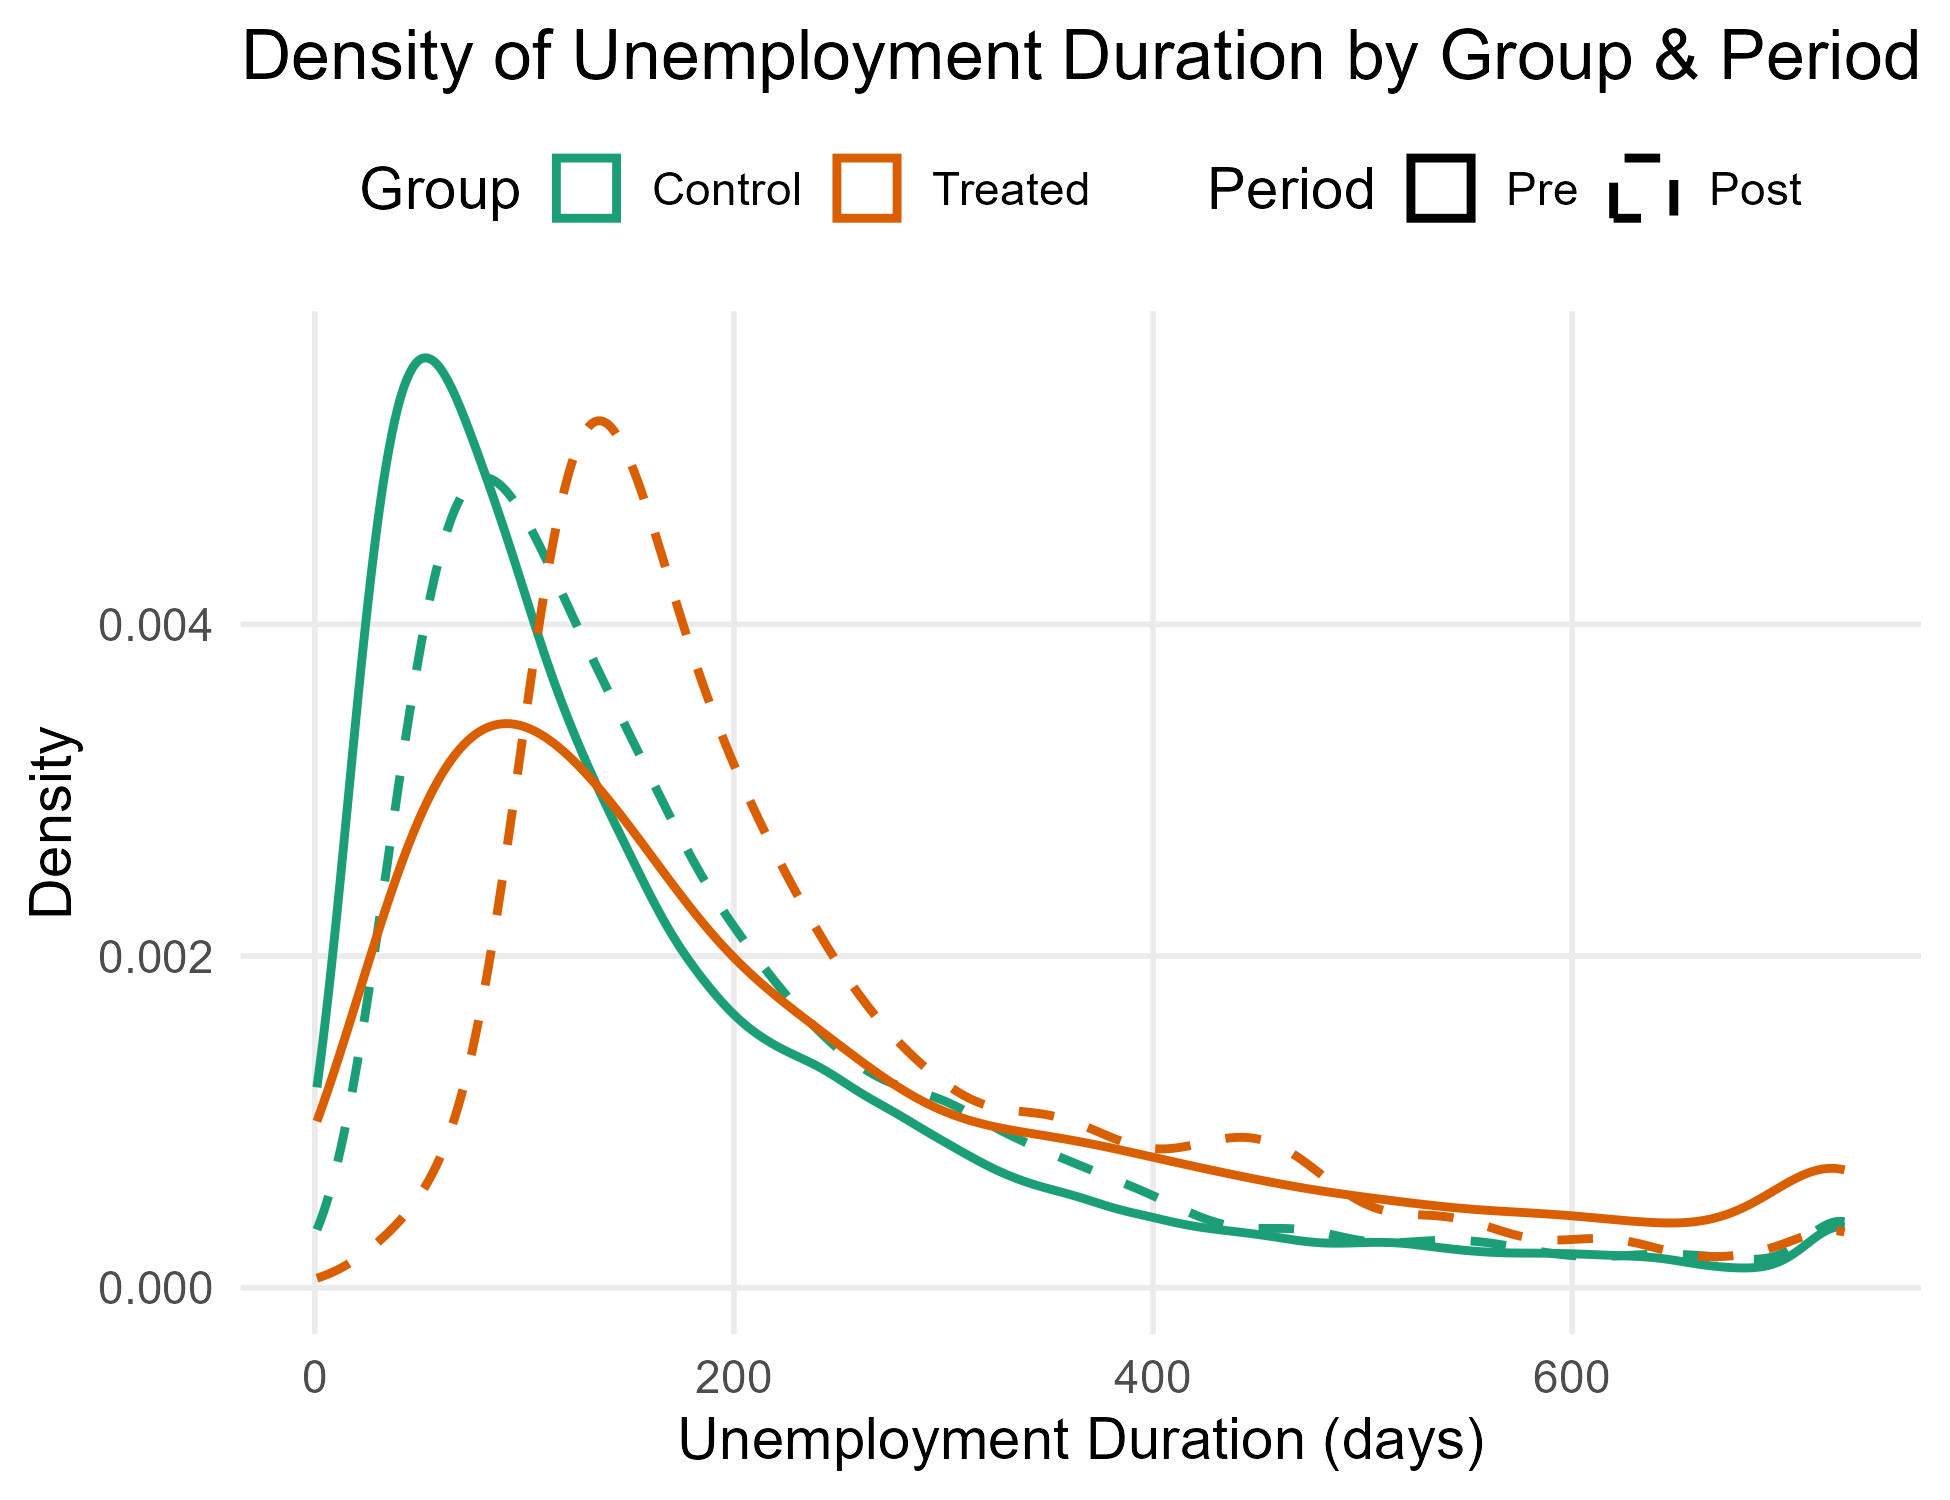
\includegraphics[width=\linewidth]{output/figures/final_unemployment_duration_density.jpg}
    \caption{Density of unemployment duration by group \& period}
    \label{fig:density}
  \end{subfigure}
  \hfill
  \begin{subfigure}[t]{0.48\textwidth}
    \centering
    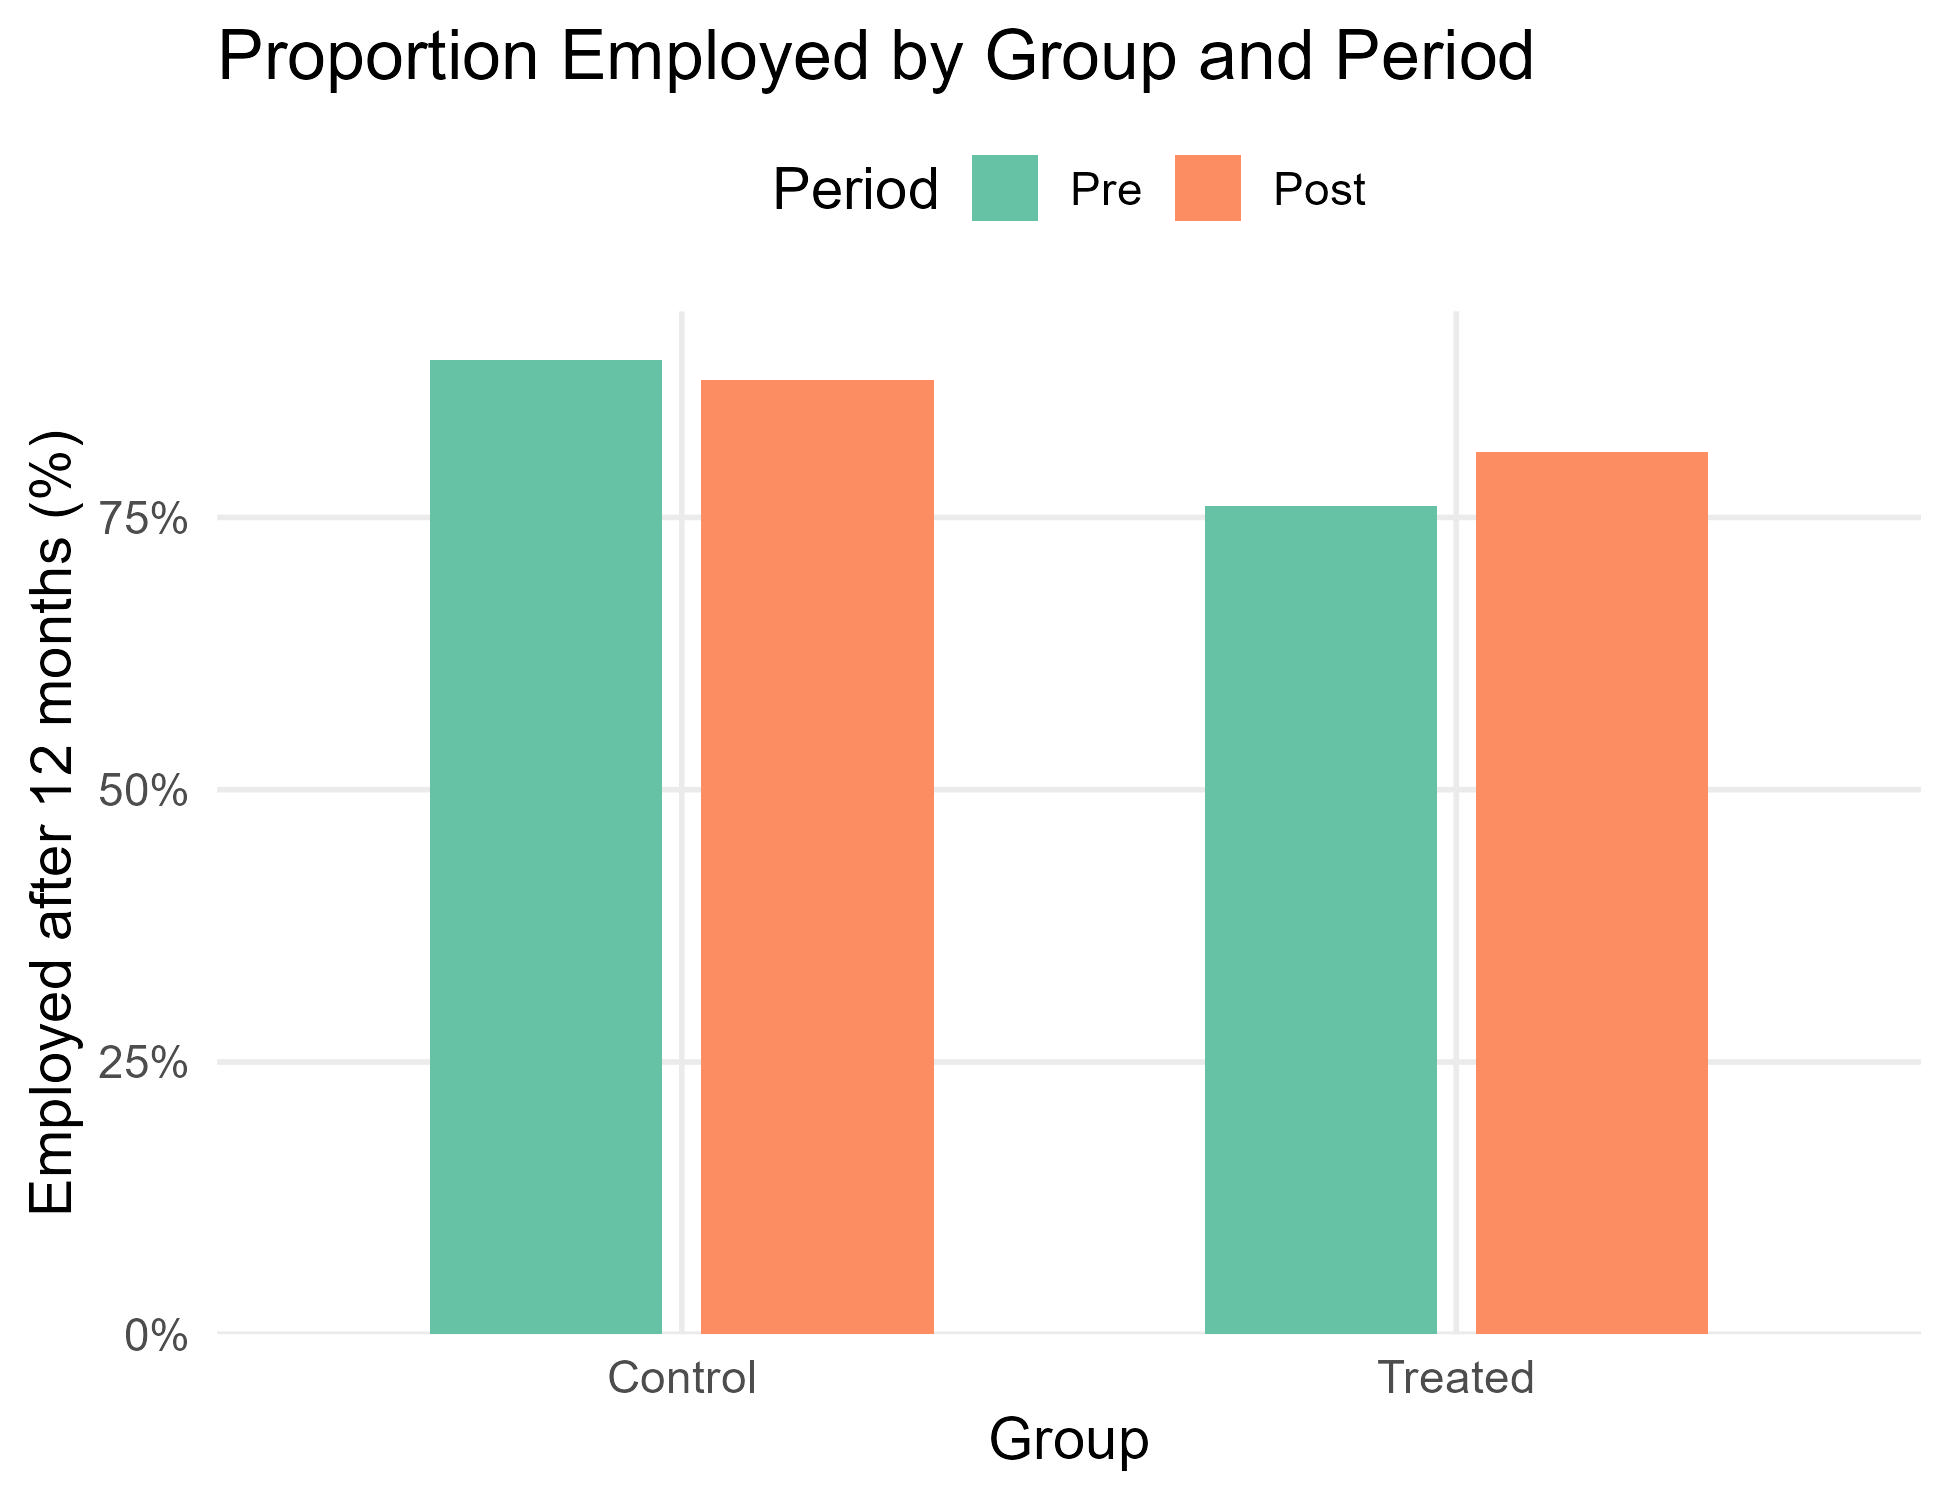
\includegraphics[width=\linewidth]{output/figures/final_employment12m.jpg}
    \caption{Proportion employed after 12 months by group \& period}
    \label{fig:employment}
  \end{subfigure}
  %–––––––––––––––––––––––––––––––––––––––––––––––––––––––––––––––––––––––––
  \caption{Visual representation of the outcome variables for the four relevant groups.}
  \label{fig:combined}
\end{figure}


Figure \ref{fig:density} shows the sample distribution of the four groups. We can see that the treated group peaks in both the pre- and post-treatment period at a later time, meaning that on average they have higher unemployment duration, possibly because taking part of the 3-month training gives people less time for job searching. Figure \ref{fig:employment} also shows that on average, the control group has a higher chance to be employed after 12 months of the start of their employment spell compared to the treated group. Nevertheless, the treated group shows an increase from pre- to post-treatment period, while the control group sees a small decrease over time. Whether this increase in employability can be attributed to the training program remains to be seen and will be analyzed later in the assignment. However, the fact that the control group sees a small decrease over time while the treated group shows an increase, already hints towards different trends for both groups, and so this warrants further investigation. \\ 


\begin{figure}[h!]
  \centering
  
  \begin{subfigure}[t]{0.48\textwidth}
    \centering
    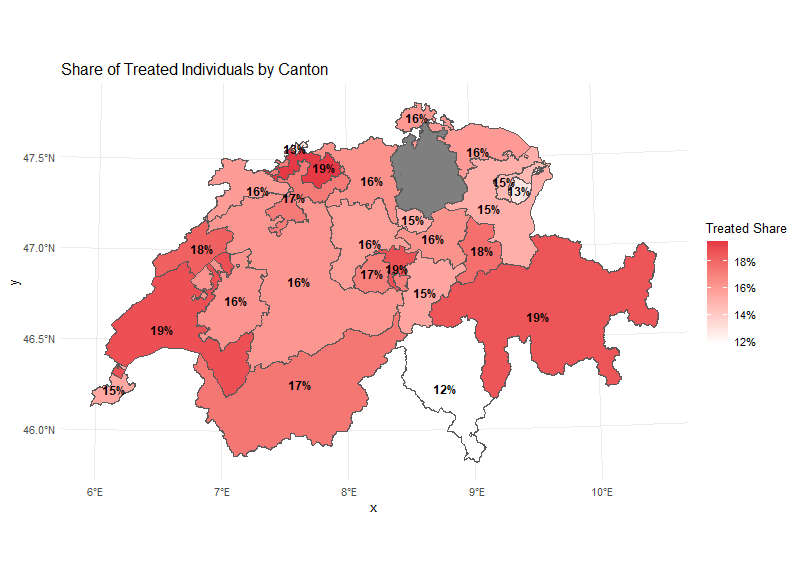
\includegraphics[width=\linewidth]{output/figures/final_map_share_treated.png}
    \caption{Share of treated units}
    \label{fig:map_treated}
  \end{subfigure}
  \hfill
  \begin{subfigure}[t]{0.48\textwidth}
    \centering
    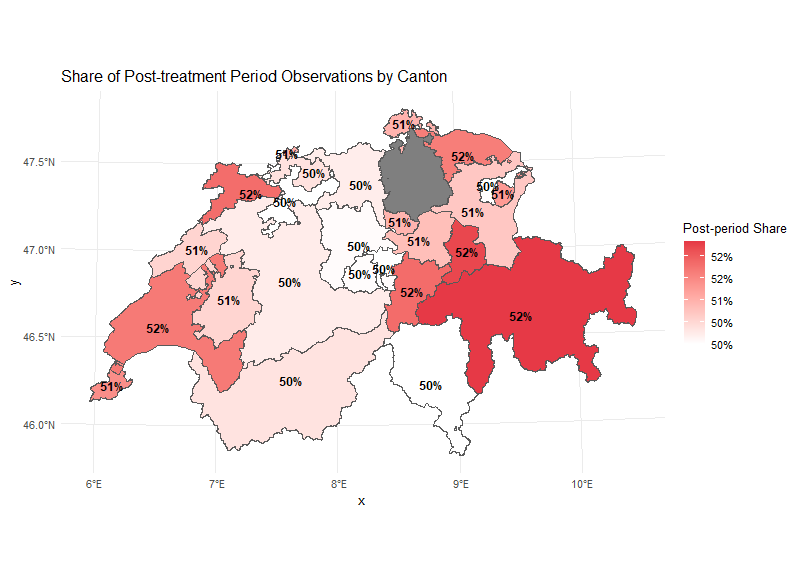
\includegraphics[width=\linewidth]{output/figures/final_map_post_share.png}
    \caption{Share of post-treatment periods}
    \label{fig:map_post}
  \end{subfigure}

  \caption{Share of Treated units and share of post-treatment units per Canton}
  \label{fig:combined2}
\end{figure}

Lastly, we wanted to investigate the share of treated vs. control units and the share of pre- vs. post-treatment periods per canton in this dataset. The dataset is notably balanced over all cantons, having between 12\% to 18\% of treated units compared to control units for all Cantons. This means that there is a somewhat equal representation from each cantons, and that treated units are not over-represented in some cantons compared to control units. We observe the same in figure \ref{fig:map_post}, with a close to equal split between pre- and post-treatment periods per canton in our dataset. One notable absence from this dataset is the Canton of Zurich, which has the highest population in Switzerland. The reason is unknown, but it might be that the training program was not offered there and was therefore excluded from the dataset.


  
\paragraph*{3.}
% Compare mean observed characteristics for all four relevant groups (treated pre/post, controls
% pre/post). Discuss the results. [6 points]

% - Maybe add education
% - Map of switzerland
Table \ref{tab:tab:final_mean_char} shows the mean observed characteristics for all four relevant groups. We note that treated people:

\begin{itemize}[label=$\blacktriangleright$]
    \item \textbf{Are older}. This is expected given how the policy has been implemented; \
    \item \textbf{Are prevalently women}. \
    \item \textbf{Have higher insured earnings.} This might reglect that they are older compared to non-treated. \
    \item \textbf{Had higher part-time rates}. \
    \item \textbf{Receive more children subsidies.} Again, this might reflect that they are older than non-treated \
    \item \textbf{Have worked a similar number of months preceding unemployment}. \ 
    \item \textbf{Have similar education levels compared to control.} This might be somewhat surprising, given the big age difference between the two groups. 
    
\end{itemize}

\begin{table}[!h]
\centering
\caption{\label{tab:final_mean_char}Mean observed characheristics by Treatment Group and Period}
\centering
\resizebox{\ifdim\width>\linewidth\linewidth\else\width\fi}{!}{
\begin{tabular}[t]{rrrrrrrrrrr}
\toprule
\multicolumn{2}{c}{ } & \multicolumn{3}{c}{Demographics} & \multicolumn{2}{c}{Economic} & \multicolumn{4}{c}{Other} \\
\cmidrule(l{3pt}r{3pt}){3-5} \cmidrule(l{3pt}r{3pt}){6-7} \cmidrule(l{3pt}r{3pt}){8-11}
Treat. & Post & N & Age (yrs) & Female (\%) & Married (\%) & Earnings & Act. rate (\%) & Child sub. (\%) & Contr. 2y (m) & Educ.\\
\midrule
0 & 0 & 8080 & 29.5 & 56.1 & 21.6 & 4482.8 & 93.1 & 6.6 & 10.8 & 1.2\\
0 & 1 & 8292 & 32.8 & 55.9 & 23.5 & 4404.0 & 88.7 & 11.0 & 10.0 & 1.1\\
1 & 0 & 3692 & 49.1 & 59.1 & 49.2 & 5285.6 & 86.5 & 9.0 & 11.8 & 1.1\\
1 & 1 & 3898 & 53.0 & 57.7 & 47.5 & 5200.5 & 82.9 & 13.6 & 10.9 & 1.1\\
\bottomrule
\end{tabular}}
\end{table}

\paragraph*{4.}
% Which assumptions do you need to identify the effect of interest based on DiD in this setup?
% [5 points]

We need:

\begin{itemize}[label=$\blacktriangleright$]
    \item \textbf{Stable unit treatment value assumption (SUTVA).} Each unit’s potential outcome under a given treatment depends only on its own treatment assignment, not on the treatments received by any other units;\
    \item \textbf{No anticipation assumption (NA)}. (Un-)Employed people do not change their behavior in anticipation of the treatment. \
    \item \textbf{Common trend assumption (CT).} Treated and controls are subject to the same time trend in the absence of treatment. \
    \item \textbf{Exogeneity assumption (EX)}. Covariates are unaffected by treatment.\ 
    \item \textbf{Common support (CS)}. Comparable observations in all groups.
\end{itemize}

\paragraph*{5.}
% Plot average outcomes for treatment and control group for each month in the observation
% period. Discuss the results. [6 points]

Figure \ref{fig:combined_overtime} shows the evolution of the outcome variables over time in the observation period. We notice that the employment rate for the treated is virtually zero in the first three months after they enter unemployment. This is likely because the program lasts 3 months, during which their ability to look for a job is arguably lower. The dashed line shows the values of the outcomes starting from the beginning of the program instead of from the beginning of the unemployment spell. Employment rates and unemployment duration mechanically appear better and more similar to the non-treated group.

\begin{figure}[h!]
  \centering
  %–––––––––––––––––––––––––––––––––––––––––––––––––––––––––––––––––––––––––
  \begin{subfigure}[t]{0.48\textwidth}
    \centering
    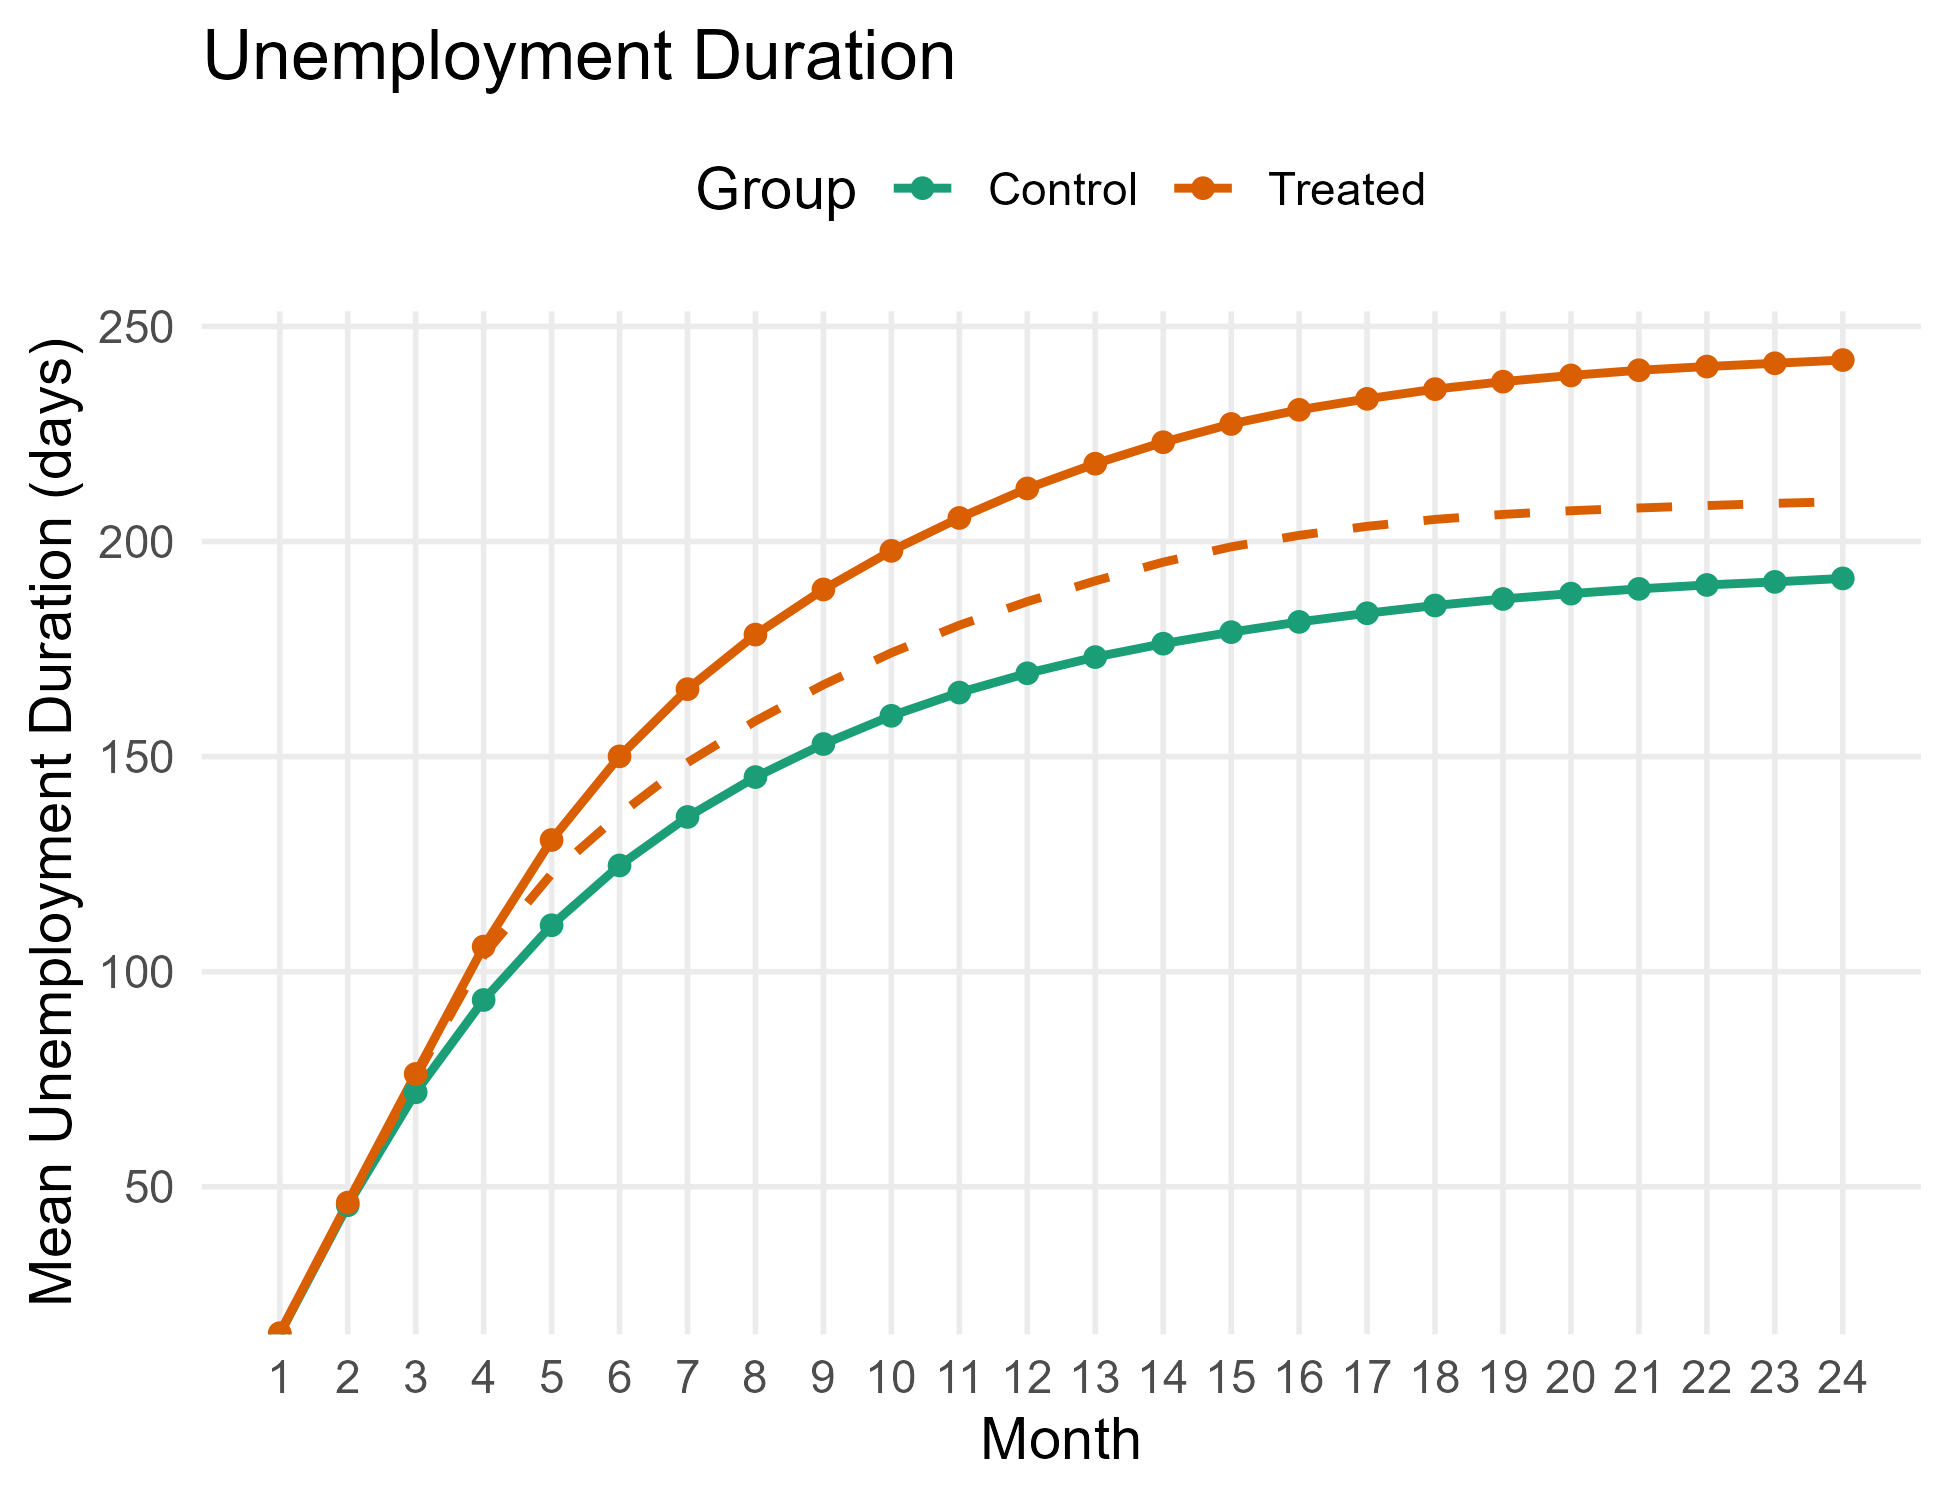
\includegraphics[width=\linewidth]{output/figures/final_unemployment_duration_over_time.jpg}
    \caption{}
    \label{fig:duration_overtime}
  \end{subfigure}
  \hfill
  \begin{subfigure}[t]{0.48\textwidth}
    \centering
    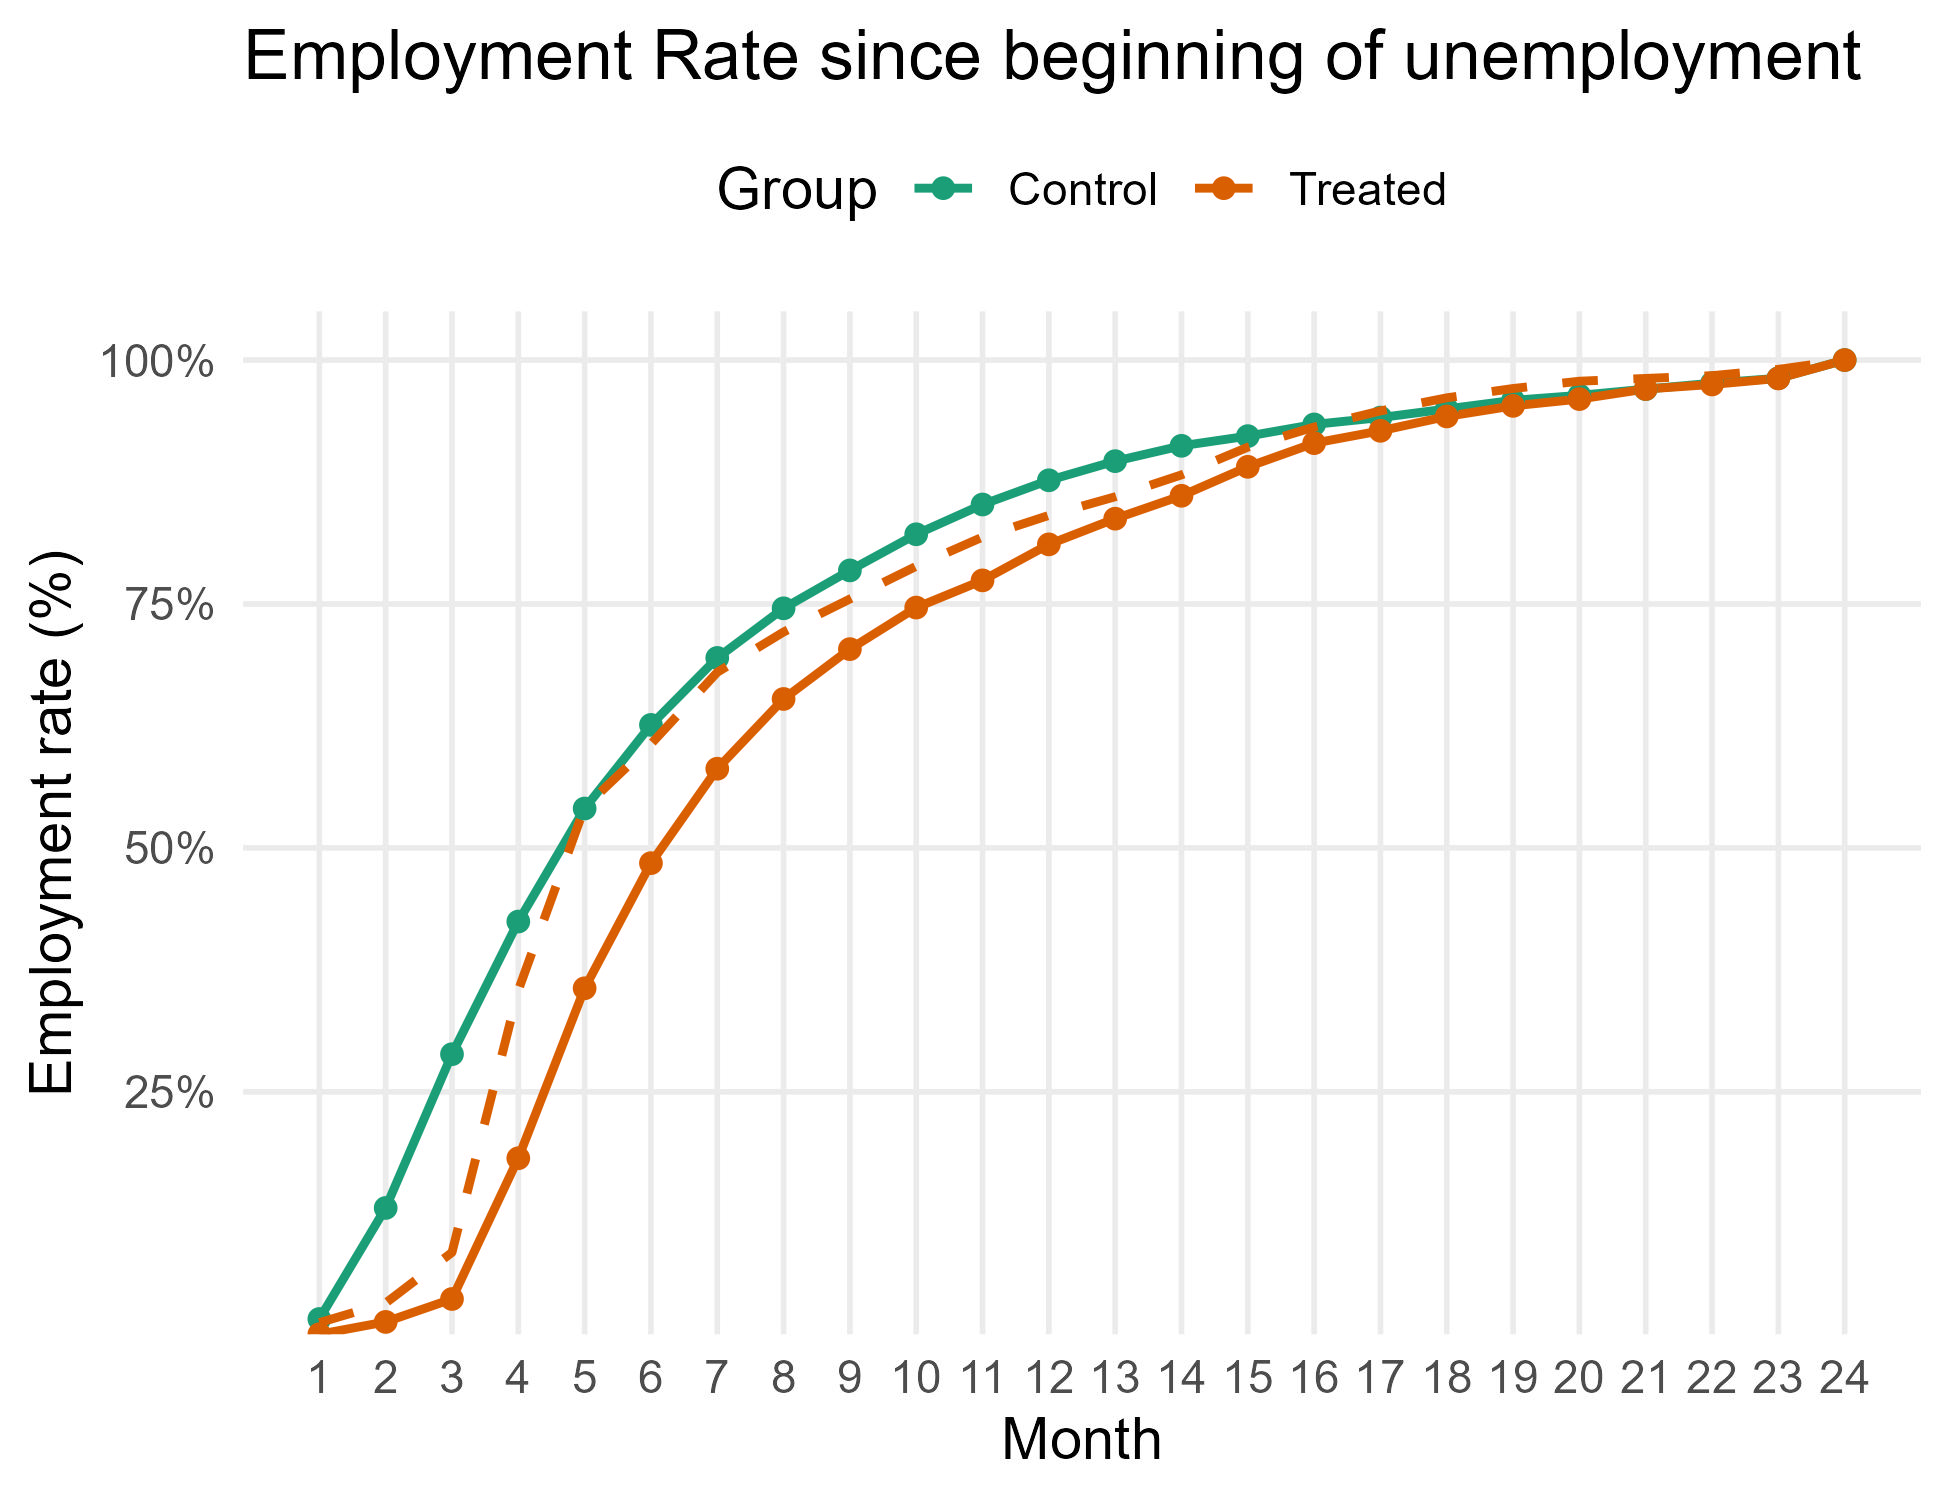
\includegraphics[width=\linewidth]{output/figures/final_employment_rate_over_time.jpg}
    \caption{Probability of being employed after x months}
    \label{fig:employment_overtime}
  \end{subfigure}
  %–––––––––––––––––––––––––––––––––––––––––––––––––––––––––––––––––––––––––
  \caption{Visual representation of the outcome variables over time in the observation period.}
  \label{fig:combined_overtime}
\end{figure}


\paragraph*{6.}
% Discuss the validity of the identifying assumptions in this specific case. Provide and discuss supporting evidence if possible, incl. event study estimates. [8 points]

\begin{itemize}[label=$\blacktriangleright$]
    \item \textbf{Stable unit treatment value assumption (SUTVA)}. SUTVA is not respected in case non-participating people are affected by those who join the program. It's possible that competition effects arise because many people apply for the same position and those who participated in the program win at the expense of others. However, it's also true that such programs might help reduce the mismatch between the skills looked for by employers and the skills of the employees. In addition, the age difference between the treatment and control groups is quite large as evidenced from figure \ref{fig:age_hist}, and table \ref{tab:tab:final_mean_char}, which specifies an average of 20 year difference. It might very well be the case that the two groups tend to apply for different kinds of jobs that require different levels of experience. If that is the case, then SUTVA is not violated, and we continue our analysis assuming that it holds.\

    \item \textbf{No anticipation assumption (NA)}. According to the text, `\textit{Prior discussions about this policy change have remained confidential, so that neither caseworkers nor the unemployed had knowledge about it before this date}. If that is true, then this assumption is respected. \

        \begin{figure}
            \centering
            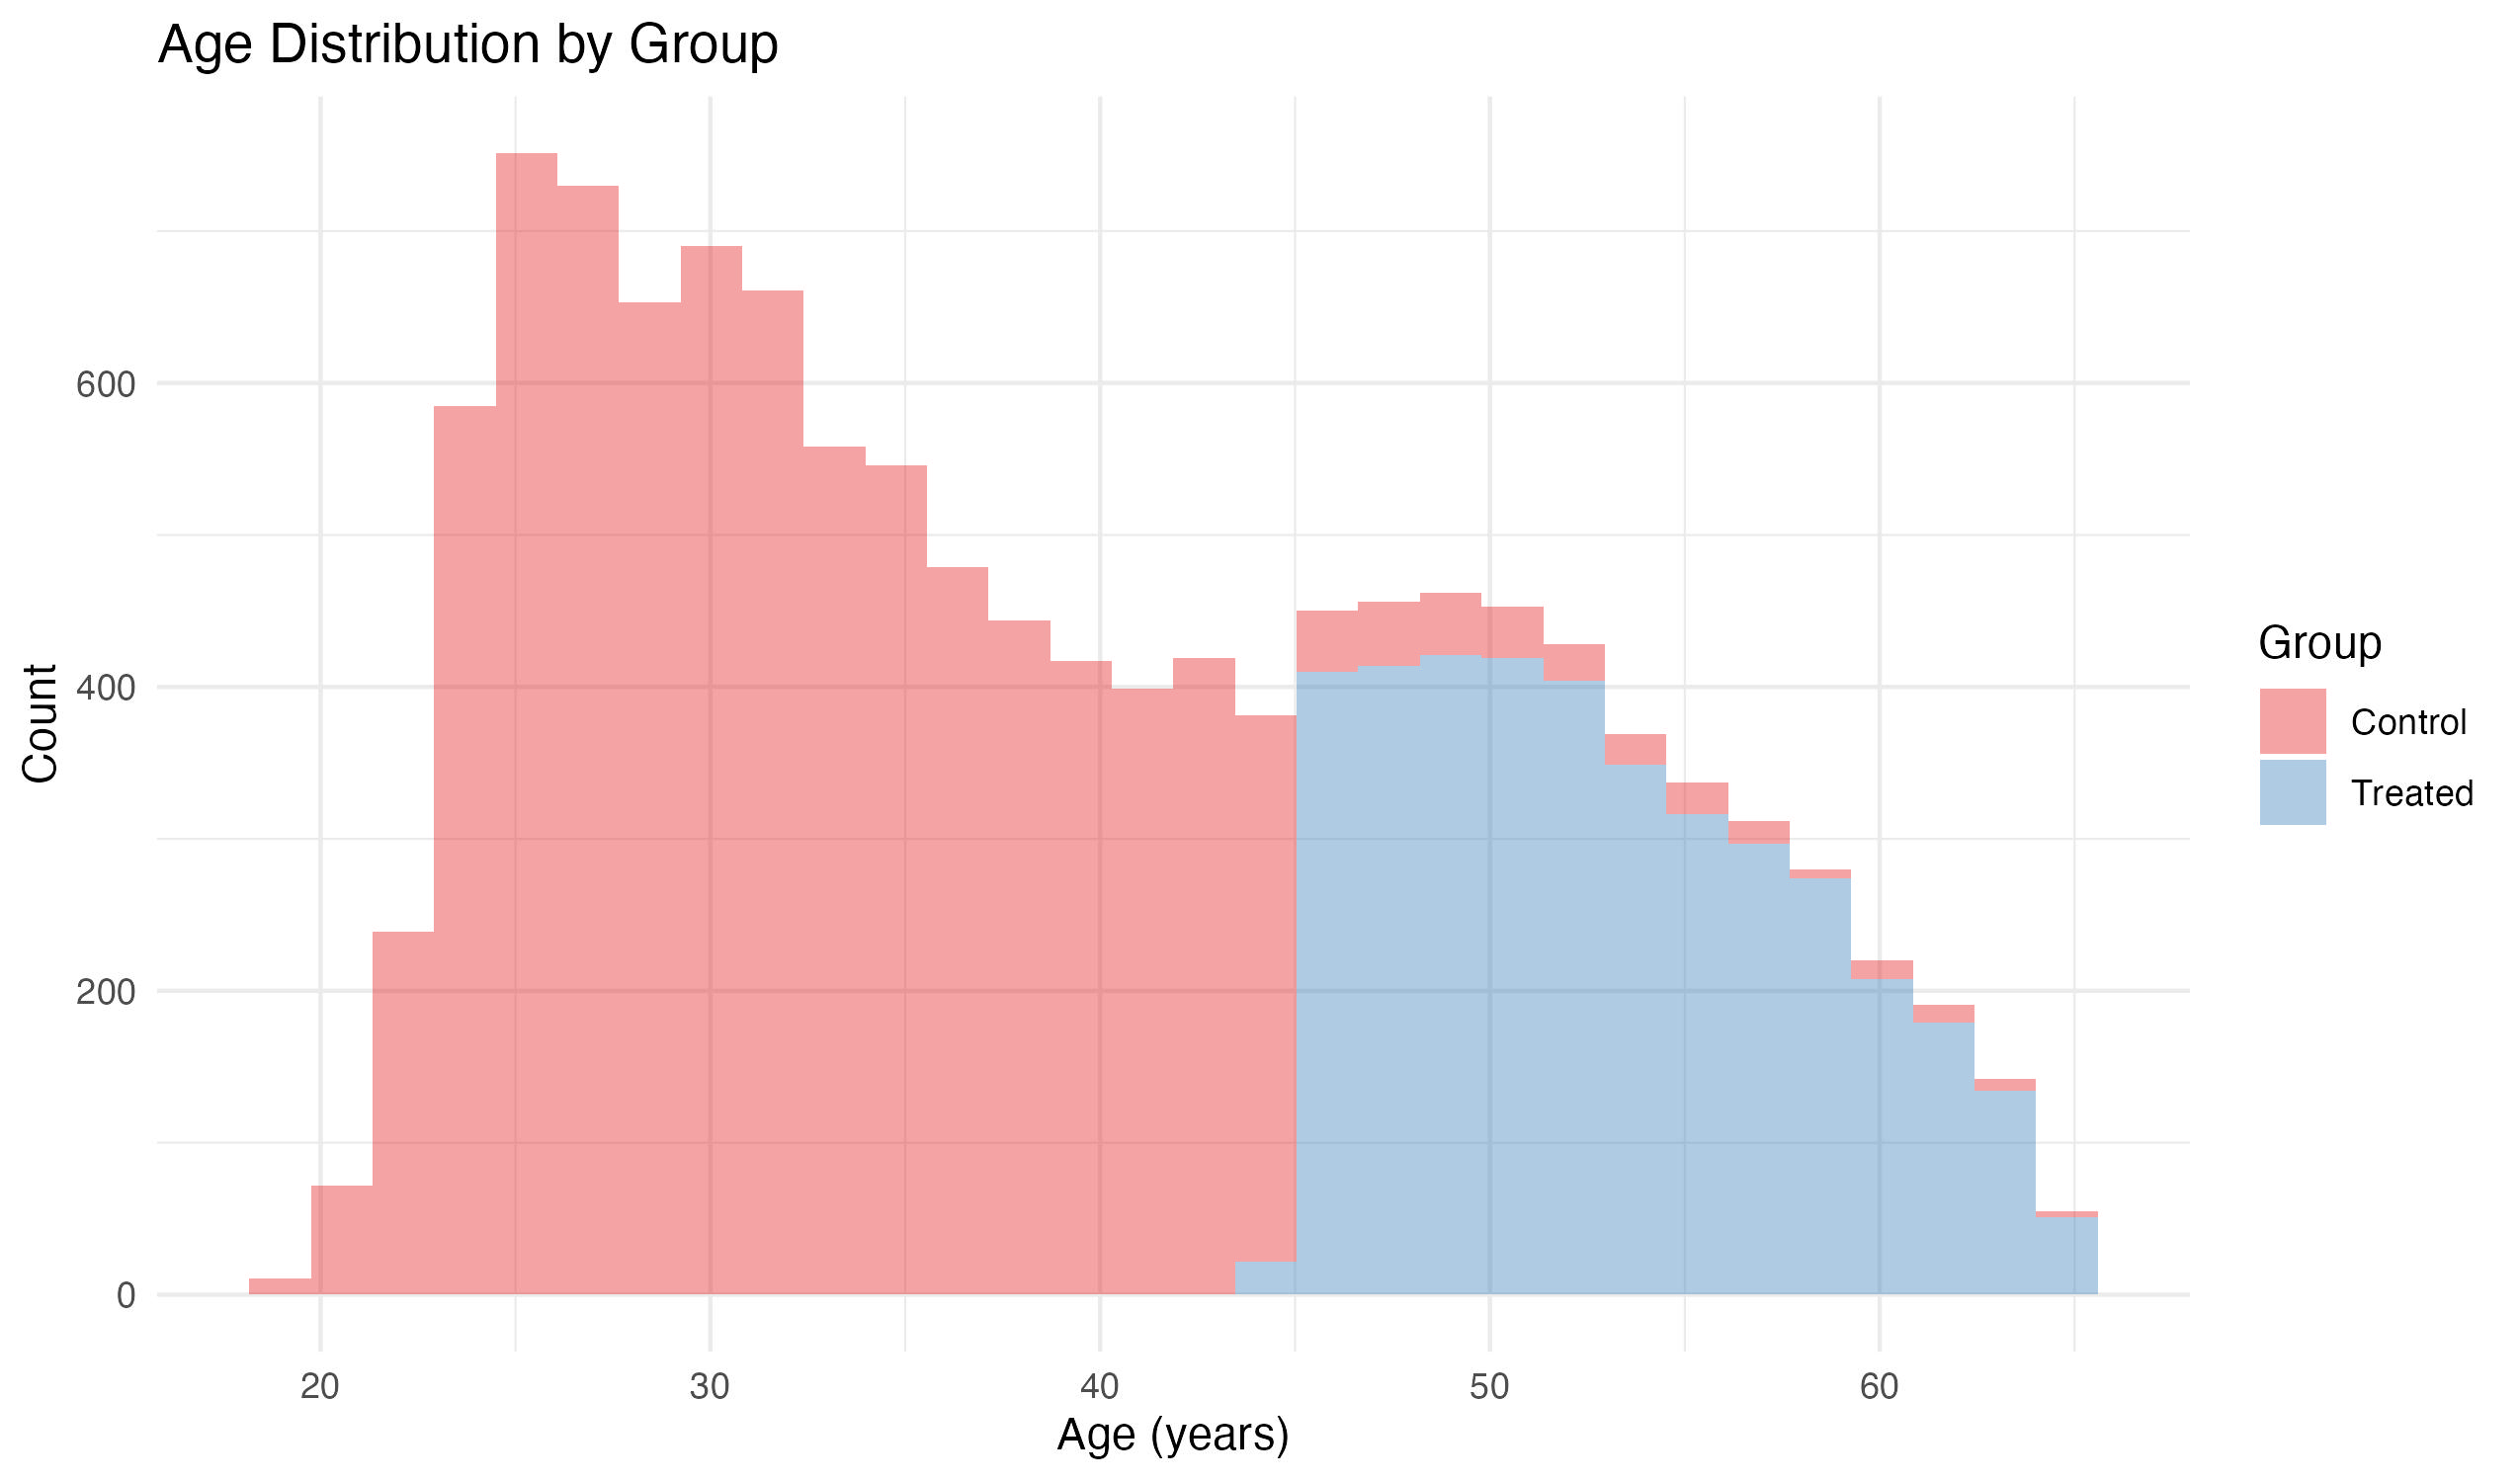
\includegraphics[width=0.75\linewidth]{output/figures/final_histogram_age.jpg}
            \caption{Age groups among treated and non-treated in the observation period.}
            \label{fig:age_hist}
        \end{figure}

    \item \textbf{Common trend assumption (CT).} Ideally we would like to present an event study to investigate pre-trends. That design needs outcomes observed reliably at several points before and after the moment treatment begins for every treated unit, so that one can plot and test the lead-lags coefficients. We only have data for two calendar years (2010 and 2015). In order to construct a multi-period outcome panel, we need to make additional, strong assumptions on the data and cannot investigate the two outcomes asked for. We believe that this approach best fits a later task description and present the results of this analysis in Figure~\ref{fig:event_study}. \\
    
    While unable to observe pre-trends and their parallelism, we want to make several theoretical statements towards the CT assumption. The task description noted that there was qualitative evidence for self-selection into treatment. Observing take-up rates within eligibility groups, we find that an overwhelming majority of those allowed to participate do take up on the opportunity. This means that at least for our data sample, self-selection appears to be limited. The central remaining issue is that our two groups of comparison mechanically differ significantly due to the fact that they are selected by age. This would break CT if the probability of reemployment decreased nonlinearly across age. If those participating in the program, who are necessarily older than the control group, had worse trends, CT is broken. In Figure~\ref{fig:age-unemp} however, we show that within the entire sample, unemployment duration increases with age in an almost perfectly linear fashion. Barring any other shocks to employment affecting the two groups differently we think that we have a good case for the CT assumption to hold, even unconditionally on covariates.
    %First and foremost, we believe that the panel structure mechanically breaks CT. The data is mainly comprised of individuals for which we have one pre and one post introduction observation. Between these two observations, individuals age by three to five, but on average about four years. We believe it is reasonable to assume that the probability of reemployment decreases with age. We also believe that decreases nonlinearly First of all, we note that the average age difference between the treatment and control group is very high. We can see this as well in figure ~\ref{fig:age_hist}, where the vast majority of people that satisfy the age requirement of >45 years, will get treated. This means that treatment and control groups are fundamentally different in their potential outcomes, since younger people are more likely to find a job and have shorter unemployment spells compared to older people. Furthermore, the prospects of finding a job for older people get significantly worse as time passes while for young people not as much (their employability from being 30 compared to 35 is relatively the same). 
    %This huge drawback means that we cannot assume that the estimates have a causal interpretation, and we will need to use extensions to the standard DiD approach in order to do causal estimation and inference. In later questions we will perform a semi-parametric DiD approach that combines matching and DiD, in order to have treatment and control groups that are more similar to each other.  We will also transform the initial dataset to allow for a staggered approach to DiD. In the 2x2 DiD setting, where we observe the unemployment spells before the treatment (in 2011) and after (in 2015), we believe it is very likely that it doesn't hold. 

        \begin{figure}
            \centering
            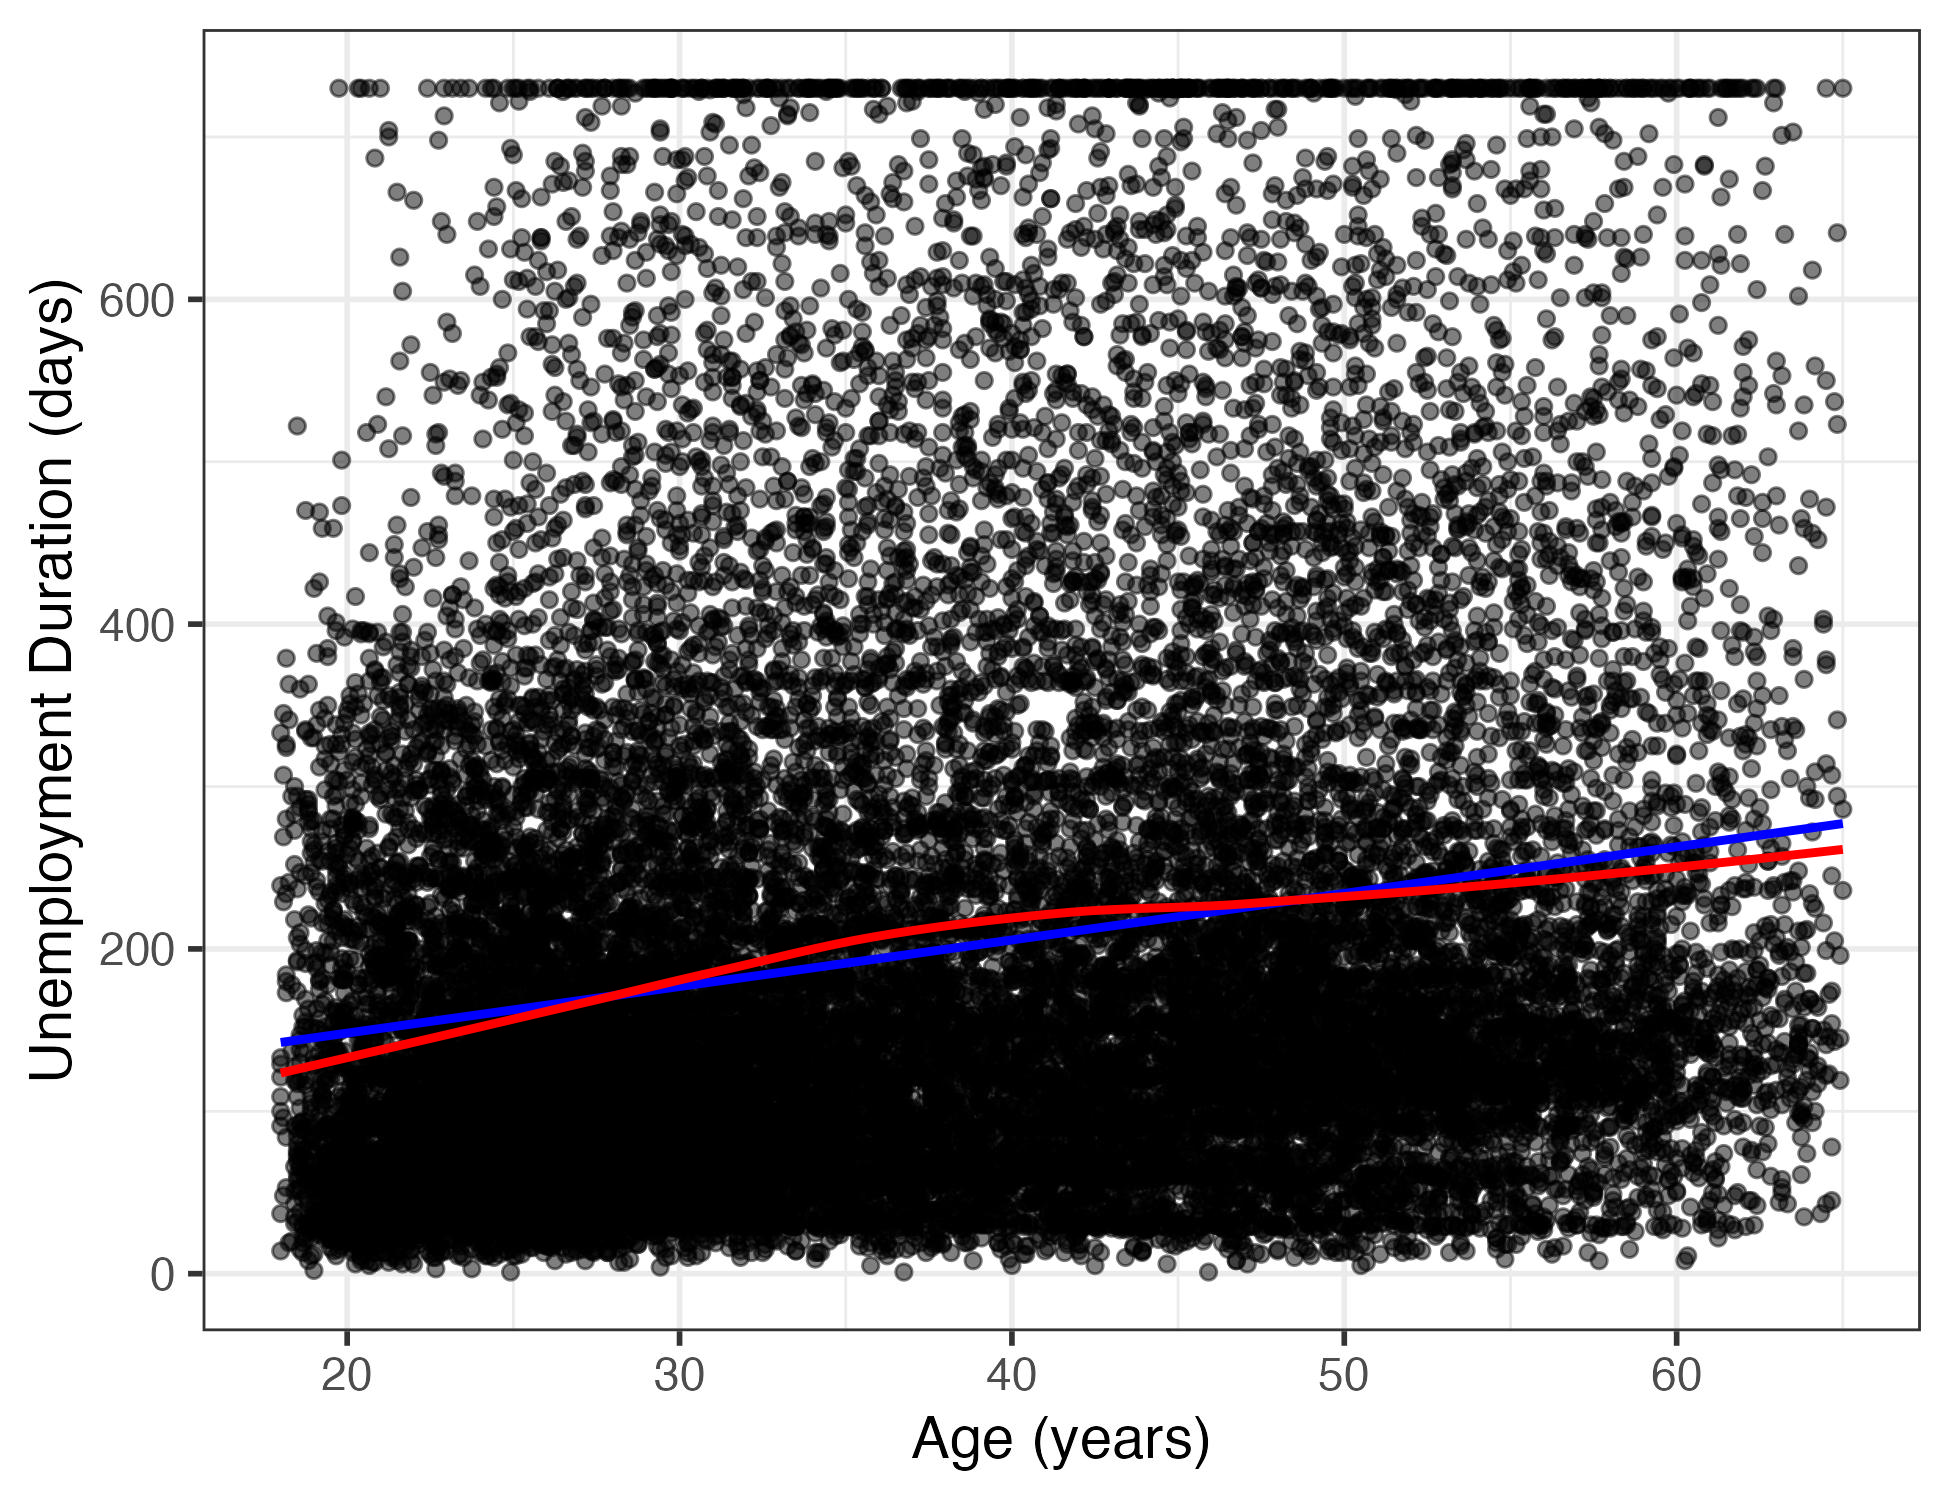
\includegraphics[width=0.75\linewidth]{output/figures/final_age_unempl_duration.jpg}
            \caption{Unemployment duration and age.}
            \label{fig:age-unemp}
        \end{figure}

    \item \textbf{Exogeneity assumption (EX)}. There is no evidence nor a compelling causal link between the treatment and the covariates in this analysis. The only plausible link would be that some people that receive the treatment (three month training) feel motivated after this training course and decide to continue their education by getting a degree. Nevertheless, we believe this to be highly unlikely, since the group that receives the treatment are above 45 years old, and are unlikely to pursue further education. 

    \item \textbf{Common support (CS)}. Treated and non-treated mechanically differ in age. Therefore, we have close to no common support in age. However, we have enough overlap in all other observable characteristics to allow us to make meaningful comparisons.
\end{itemize}

\paragraph*{7.}
% Implement the DiD using OLS. Describe in detail what you do and why. Discuss whether or
% not you need additional control variables and if so, why. Discuss the results. [8 points]

We estimate the model
$$
Y_{it} = \alpha + \beta_1 \text{Treat}_i + \beta_2 \text{Post}_t + \beta_3 (\text{Treat}_i \times \text{Post}_t) + \epsilon_{it}
$$
where \( Y_{it} \) is the outcome of interest for unit \( i \) at time \( t \), \( \text{Treat}_i \) is an indicator variable equal to 1 if the unit belongs to the treatment group, \( \text{Post}_t \) is an indicator equal to 1 for the post-treatment period, and the interaction term \( \text{Treat}_i \times \text{Post}_t \) captures the difference-in-differences (DiD) estimator \( \beta_3 \), which is our main coefficient of interest. \\

We estimate the model using Ordinary Least Squares (OLS). Nevertheless, we believe that, for the reasons stated above, the common trends assumption does not hold, and so this estimate may not accurately estimate the ATT. Adding covariates does help to increase precision and help control for residual confounding, but it doesn't tackle our main issue which is that we cannot assume parallel trends. We will however we also present results controlling for the covariates.


\begin{table}
\caption{OLS Results for Unemployment Duration and Employment After 12 Months}
\begin{center}
\begin{threeparttable}
\begin{tabular}{l D{.}{.}{5.5} D{.}{.}{5.5} D{.}{.}{5.5} D{.}{.}{5.5}}
\toprule
 & \multicolumn{2}{c}{Unemployment Duration} & \multicolumn{2}{c}{Employment After 12 Months} \\
\cmidrule(lr){2-3} \cmidrule(lr){4-5}
 & \multicolumn{1}{c}{(1a)} & \multicolumn{1}{c}{(1b)} & \multicolumn{1}{c}{(2a)} & \multicolumn{1}{c}{(2b)} \\
\midrule
(Intercept)    & 164.06^{***}         & 127.44^{***}                   & 0.89^{***}           & 1.00^{***}                     \\
               & (1.72)               & (11.69)                        & (0.00)               & (0.02)                         \\
Treated        & 78.80^{***}          & 40.96^{***}                    & -0.13^{***}          & -0.04^{***}                    \\
               & (3.72)               & (5.68)                         & (0.01)               & (0.01)                         \\
Post           & 27.36^{***}          & 21.68^{***}                    & -0.02^{***}          & -0.01^{*}                      \\
               & (0.72)               & (1.19)                         & (0.00)               & (0.00)                         \\
Treated * Post & -28.03^{***}         & -28.26^{***}                   & 0.07^{***}           & 0.07^{***}                     \\
               & (1.54)               & (1.54)                         & (0.00)               & (0.00)                         \\
\midrule
Controls       & \multicolumn{1}{c}{} & \multicolumn{1}{c}{\checkmark} & \multicolumn{1}{c}{} & \multicolumn{1}{c}{\checkmark} \\
R$^2$          & 0.04                 & 0.05                           & 0.02                 & 0.04                           \\
Adj. R$^2$     & 0.04                 & 0.05                           & 0.02                 & 0.04                           \\
Num. obs.      & 23855                & 23855                          & 23855                & 23855                          \\
\bottomrule
\end{tabular}
\begin{tablenotes}[flushleft]
\scriptsize{Covariates include age, gender, marital status, earning insured by unemployment insurance, activity rate in the last job, receiving child subsidies, months of employment in the 2 years prior to unemployment. Standard errors clustered at the individual level. $^{***}p<0.01$; $^{**}p<0.05$; $^{*}p<0.1$}
\end{tablenotes}
\end{threeparttable}
\label{tab:final_ols_results_combined}
\end{center}
\end{table}


\paragraph*{8.} 
% Implement the DiD using a semi-parametric estimator based on the propensity score. Describe
% in detail what you do and why. Discuss the results and compare them to the OLS estimates.
% [10 points]
The problem of normal parametric diff-in-diff is that if (i) individual characteristics are associated with the outcome variable and (ii) characteristics are imbalanced over the groups, it's likely that the common trend assumption does not hold. The semi-parametric DiD estimator offers a more flexible and robust estimator, as it relies on more relaxed versions of the identifying assumptions (e.g. conditional parallel trends). This approach allows us to weight observations in the control more if their covariates are more similar to those in the treatment group, and give less weight to those observations that are very different. The steps are as follows:
% We can check if the weighted average age is the same between control and treatment 

\begin{enumerate}
    \item First step: We define comparison groups. The treated group $(T=1,D=1)$ is compared to:
    \begin{itemize}
        \item Control group after treatment $(T=1,D=0)$.
        \item Control group before treatment $(T=0,D=0)$.
        \item Treated group before treatment $(T=0,D=1)$.
    \end{itemize}
    \item Second step: We estimate three propensity score models. For each pair of samples (always including $T=1,D=1$), we estimate a probit model.
    \item Third step: Estimate propensity scores and calculate weights using inverse probability weighting.
    \item Fourth step: Calculate ATET: \[
\mathbb{E}[Y \mid T=1, D=1] 
- \mathbb{E}[Y(0,1) \mid T=1] 
- \mathbb{E}[Y(1,0) \mid T=1] 
+ \mathbb{E}[Y(0,0) \mid T=1]
\]
\end{enumerate}

\begin{table}
\centering
\caption{ATET Results}
\centering
\resizebox{\ifdim\width>\linewidth\linewidth\else\width\fi}{!}{
\begin{tabular}[t]{lccccc}
\toprule
Outcome & ATET & $E[Y|T=1,D=1]$ & $E[Y(0,1)|T=1]$ & $E[Y(1,0)|T=1]$ & $E[Y(0,0)|T=1]$\\
\midrule
Unemployment Duration & -35.45 & 242.18 & 235.91 & 175.60 & 133.87\\
Employment after 12 months & 0.05 & 0.81 & 0.77 & 0.94 & 0.95\\
\bottomrule
\end{tabular}}
\end{table}


It is worth mentioning that \textit{age} alone is a good predictor of the propensity score. In fact, the treated and control groups differ mainly in their age. As it consequently is in general quite difficult to find a precise counterfactual for the treated units, the propensity score models weigh the age characteristic much more than other observable characteristics. This is quite visible by plotting, in Figure \ref{fig:prop_scores}, the relationship between the propensity score and age, for the three groups that are used in comparison with the post and treated units. 

\begin{figure}
    \centering
    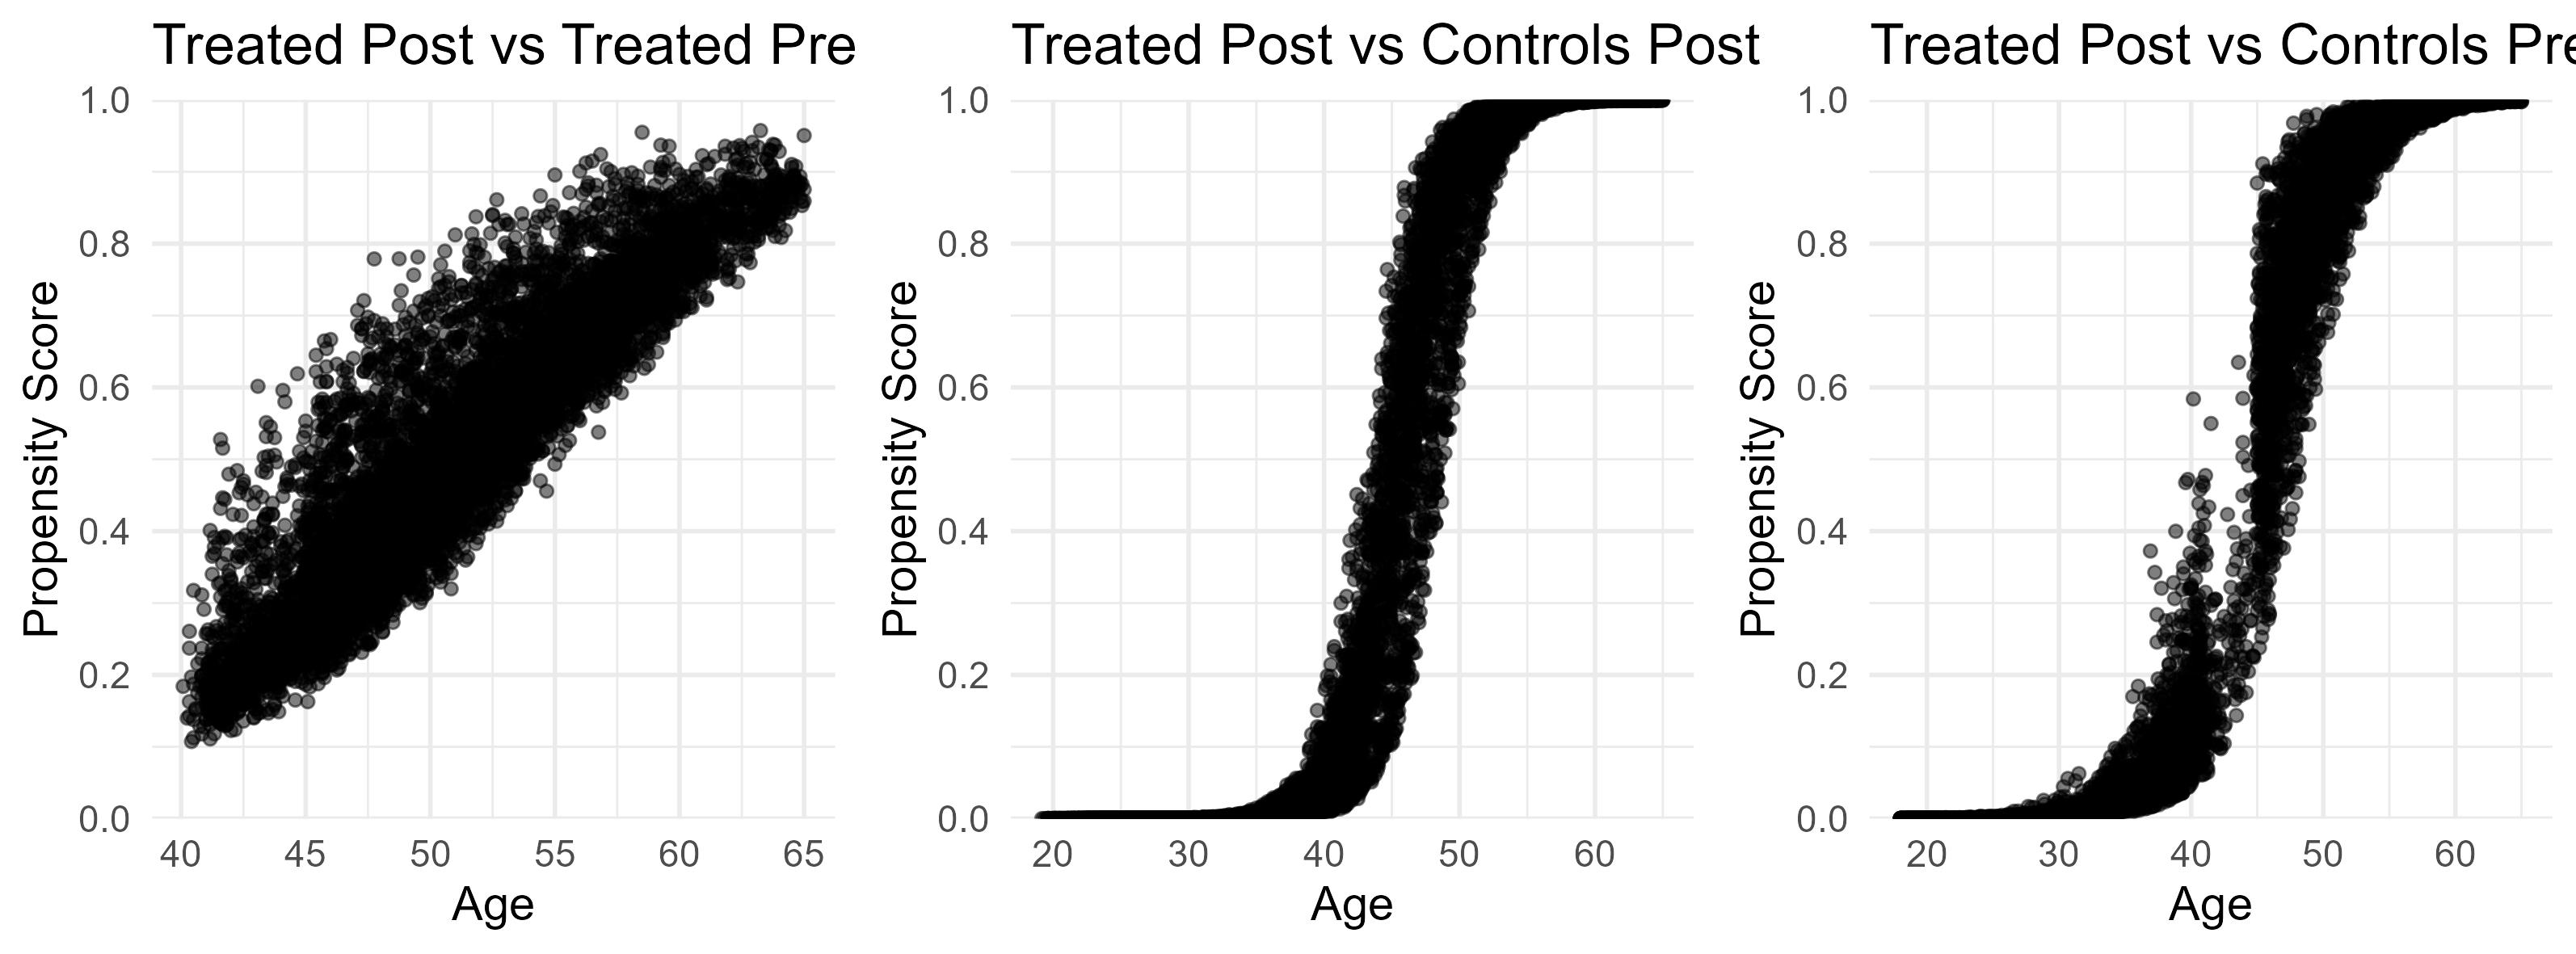
\includegraphics[width=0.8\linewidth]{output/figures/final_propensity_scores.jpg}
    \caption{Relationship between propensity score and age}
    \label{fig:prop_scores}
\end{figure}


\paragraph*{9.}
% Discuss different ways of exploiting the panel structure of the data and implement one of them.
% Discuss to which extent the panel approach relaxes assumptions underlying the estimation
% approaches you used before. Describe in detail what you do and why. Discuss the results and
% compare them the other estimates. [10 points

The existing panel structure of the data only only allows for limited extensions. The main challenge is that the data is indexed by unemployment spell. In order to turn this into a full, balanced panel at the individual level with monthly observations, we need to assume that at least for the 2015 period, we have information about all unemployment spells of the individuals. In other words, we should be able to safely assume that any period not covered in the data means the individual is employed. Doing that, we are able to transform the data into such a panel where the outcome variable is the binary employment status and we have cross-sectional demographic information.

The resulting panel allows us to investigate treatment effects on employment status at arbitrary temporary lags and leads. Because actual treatment months differ, we employ the \cite{callawayDifferenceinDifferencesMultipleTime2020} estimator, which accounts for the potential negative weights problem. This regresses employment on leads and lags of treatment with the program per treatment cohort, using the never treated as the control group. Then, we aggregate the results into a plot, employing the robust cohorts weights implement in the R package accompanying the estimator. We present our results in an event-study plot in Figure~\ref{fig:event_studies}.

\begin{figure}[h!]
  \centering
  
  \begin{subfigure}[t]{0.48\textwidth}
    \centering
    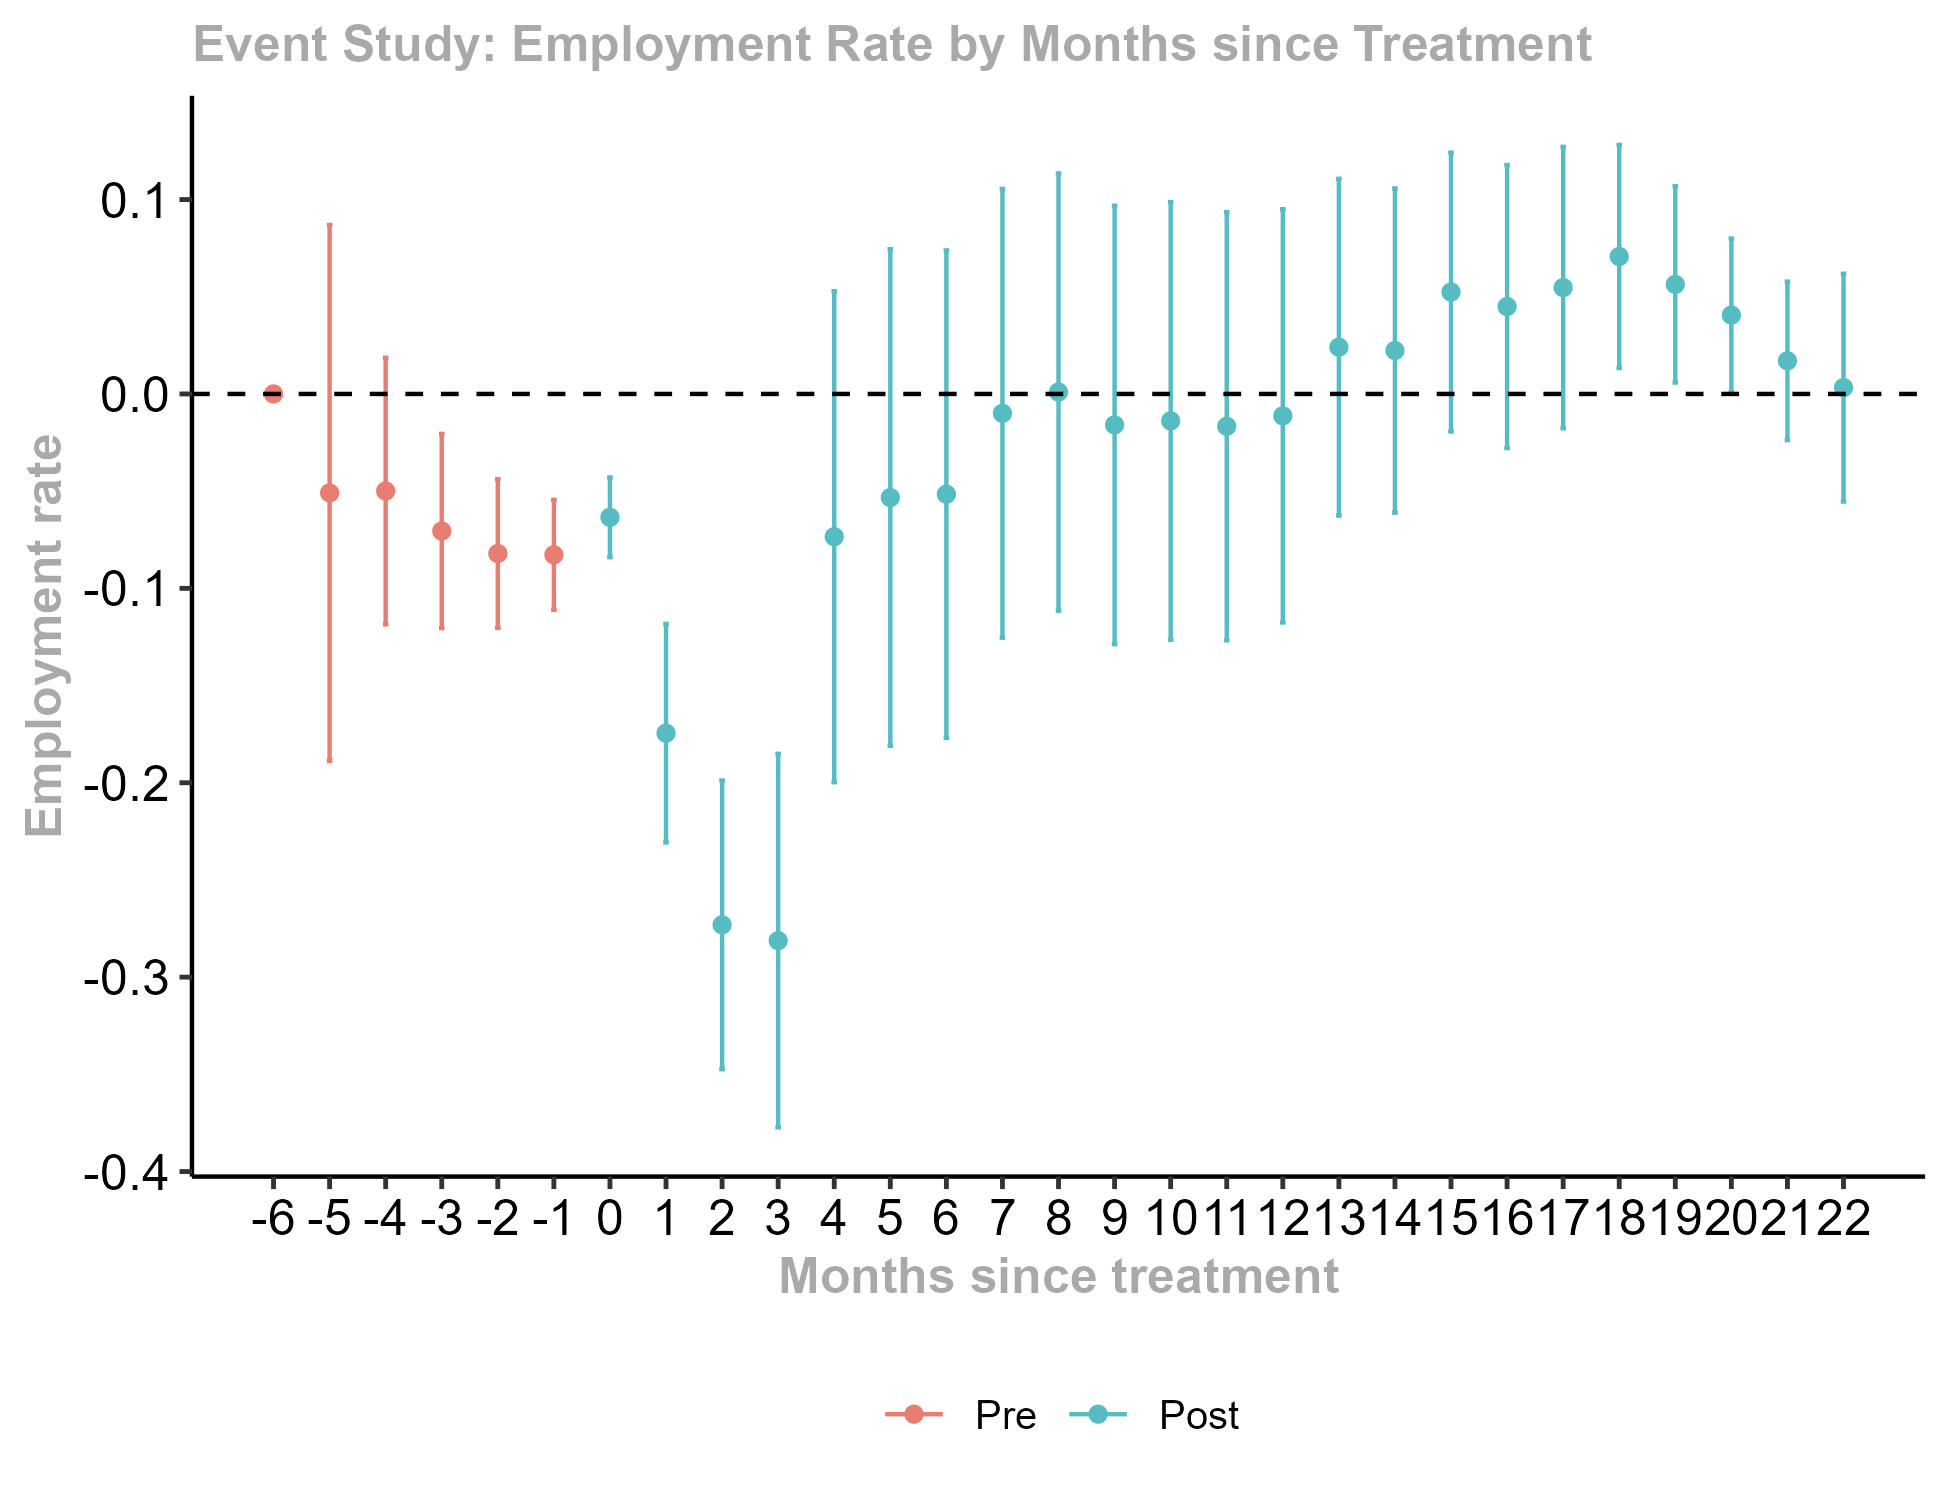
\includegraphics[width=\linewidth]{output/figures/final_event_study_employment_rate.jpg}
    %\caption{Training program and employment: Event Study.}
    \label{fig:event_study}
  \end{subfigure}
  \hfill
  \begin{subfigure}[t]{0.48\textwidth}
    \centering
    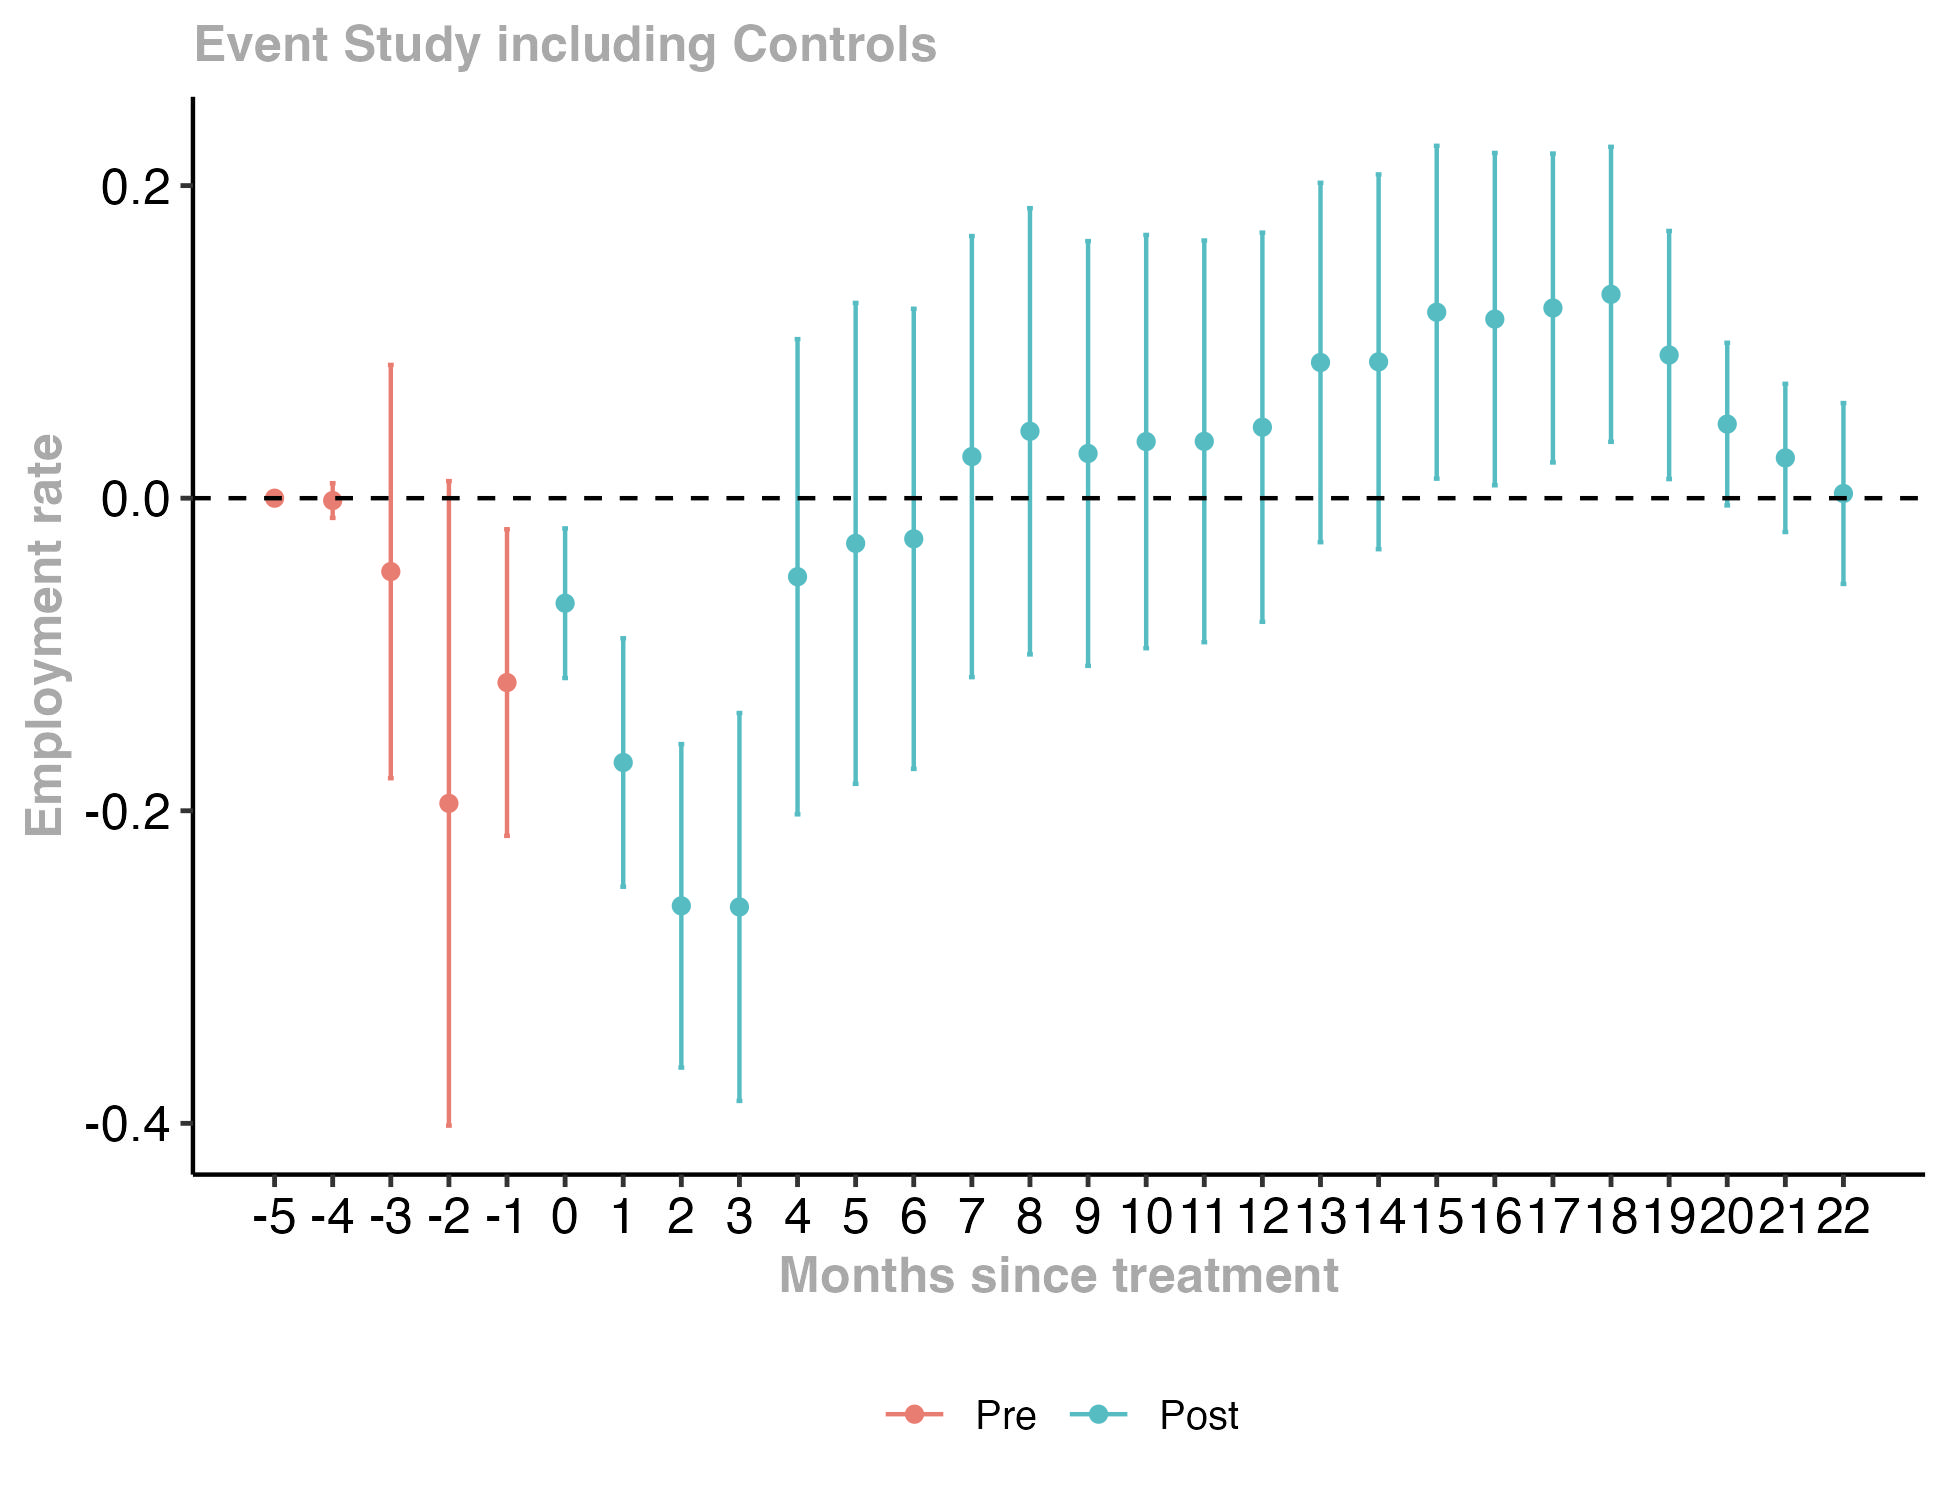
\includegraphics[width=\linewidth]{output/figures/final_event_study_employment_rate_controls.jpg}
    %\caption{Training program and employment: Event Study.}
    \label{fig:event_study_controls}
  \end{subfigure}

  \caption{Training program and employment: Event Studies}
  \label{fig:event_studies}
\end{figure}

\paragraph*{10.}
% Check for heterogeneous program effects with respect to observed characteristics for which
% you suspect different effects. Describe in detail what you do and why. Discuss the results. [5
% points]

We would like to check for spatial heterogeneous effects, since it would be natural to assume that the effect of such a training is higher for regions that are further into the transition of the digitization of the economy. Therefore, we expect cantons like Basel or Geneva to experience a stronger effect of the training program compared to more rural cantons like Uri or Glarus. We will use the standard OLS 2x2 DID model to check for heterogeneous effects. Even though we believe that the model does not accurately estimate the treatment effect, due to the common trend assumption not holding, it easy to use this model to check for heterogeneous effects, since we only need to interact the treatment coefficient $(Treat_i  \times Post_t)$, with the variable that we suspect the effect to differ for, i.e., Canton or Region. Furthermore, we are not interested in the estimate itself, but rather, if the model is able to significantly distinguish different effects per canton or region, which is why we chose this simple model to check for heterogenous effect over the more complicated DiD extensions we have also used (Semi-parametric DiD or Callaway \& Sant'Anna DiD estimator).

\begin{table}[!h]
\centering
\caption{Heterogeneous Effects per Region: Unempl. Duration and Employment After 12 Months}
\label{tab:heterogeneous_region}
\centering
\resizebox{\ifdim\width>\linewidth\linewidth\else\width\fi}{!}{
\begin{tabular}[t]{lccc|ccclccc|ccclccc|ccclccc|ccclccc|ccclccc|ccclccc|ccc}
\toprule
\multicolumn{1}{c}{ } & \multicolumn{3}{c}{Unempl. Duration} & \multicolumn{3}{c}{Employed After 12m} \\
\cmidrule(l{3pt}r{3pt}){2-4} \cmidrule(l{3pt}r{3pt}){5-7}
Term & Estimate & SE & p & Estimate & SE & p\\
\midrule
\cellcolor{gray!10}{$Treat_i \times Post_t \times Lake Geneva$} & \cellcolor{gray!10}{-9.229} & \cellcolor{gray!10}{5.203} & \cellcolor{gray!10}{0.076} & \cellcolor{gray!10}{0.002} & \cellcolor{gray!10}{0.015} & \cellcolor{gray!10}{0.868}\\
$Treat_i \times Post_t \times Mittelland$ & 0.904 & 4.093 & 0.825 & -0.021 & 0.012 & 0.077\\
\cellcolor{gray!10}{$Treat_i \times Post_t \times North-Western Switzerland$} & \cellcolor{gray!10}{4.781} & \cellcolor{gray!10}{4.599} & \cellcolor{gray!10}{0.299} & \cellcolor{gray!10}{-0.011} & \cellcolor{gray!10}{0.014} & \cellcolor{gray!10}{0.415}\\
$Treat_i \times Post_t \times Oriental Switzerland$ & 2.442 & 5.109 & 0.633 & -0.013 & 0.014 & 0.367\\
\cellcolor{gray!10}{$Treat_i \times Post_t \times Ticino$} & \cellcolor{gray!10}{-9.803} & \cellcolor{gray!10}{27.914} & \cellcolor{gray!10}{0.725} & \cellcolor{gray!10}{-0.079} & \cellcolor{gray!10}{0.007} & \cellcolor{gray!10}{0.000}\\
\bottomrule
\end{tabular}}
\end{table}



\begin{table}[!h]
\centering
\caption{Heterogeneous Effects per Canton: Unempl. Duration and Employment After 12 Months} \label{tab:heterogeneous_canton}
\centering
\resizebox{\ifdim\width>\linewidth\linewidth\else\width\fi}{!}{
\begin{tabular}[t]{lccc|ccclccc|ccclccc|ccclccc|ccclccc|ccclccc|ccclccc|ccc}
\toprule
\multicolumn{1}{c}{ } & \multicolumn{3}{c}{Unempl. Duration} & \multicolumn{3}{c}{Employed After 12m} \\
\cmidrule(l{3pt}r{3pt}){2-4} \cmidrule(l{3pt}r{3pt}){5-7}
Term & Estimate & SE & p & Estimate & SE & p\\
\midrule
$Treat_i \times Post_t \times AI$ & 35.941 & 38.218 & 0.347 & 0.127 & 0.182 & 0.485\\
\cellcolor{gray!10}{$Treat_i \times Post_t \times AR$} & \cellcolor{gray!10}{39.362} & \cellcolor{gray!10}{23.008} & \cellcolor{gray!10}{0.087} & \cellcolor{gray!10}{-0.041} & \cellcolor{gray!10}{0.037} & \cellcolor{gray!10}{0.264}\\
$Treat_i \times Post_t \times BE$ & -5.593 & 6.542 & 0.393 & -0.002 & 0.019 & 0.908\\
\cellcolor{gray!10}{$Treat_i \times Post_t \times BL$} & \cellcolor{gray!10}{-15.061} & \cellcolor{gray!10}{9.062} & \cellcolor{gray!10}{0.097} & \cellcolor{gray!10}{-0.004} & \cellcolor{gray!10}{0.026} & \cellcolor{gray!10}{0.887}\\
\addlinespace
$Treat_i \times Post_t \times BS$ & -21.580 & 11.430 & 0.059 & 0.048 & 0.040 & 0.233\\
\cellcolor{gray!10}{$Treat_i \times Post_t \times FR$} & \cellcolor{gray!10}{-27.631} & \cellcolor{gray!10}{9.117} & \cellcolor{gray!10}{0.002} & \cellcolor{gray!10}{0.000} & \cellcolor{gray!10}{0.028} & \cellcolor{gray!10}{0.998}\\
$Treat_i \times Post_t \times GE$ & -25.911 & 8.853 & 0.003 & 0.017 & 0.026 & 0.515\\
\cellcolor{gray!10}{$Treat_i \times Post_t \times GL$} & \cellcolor{gray!10}{30.488} & \cellcolor{gray!10}{24.540} & \cellcolor{gray!10}{0.214} & \cellcolor{gray!10}{-0.087} & \cellcolor{gray!10}{0.031} & \cellcolor{gray!10}{0.005}\\
$Treat_i \times Post_t \times GR$ & 8.603 & 9.418 & 0.361 & 0.027 & 0.032 & 0.398\\
\addlinespace
\cellcolor{gray!10}{$Treat_i \times Post_t \times JU$} & \cellcolor{gray!10}{-28.526} & \cellcolor{gray!10}{17.112} & \cellcolor{gray!10}{0.096} & \cellcolor{gray!10}{-0.013} & \cellcolor{gray!10}{0.057} & \cellcolor{gray!10}{0.813}\\
$Treat_i \times Post_t \times LU$ & -10.832 & 9.273 & 0.243 & -0.032 & 0.025 & 0.208\\
\cellcolor{gray!10}{$Treat_i \times Post_t \times NE$} & \cellcolor{gray!10}{-20.140} & \cellcolor{gray!10}{12.678} & \cellcolor{gray!10}{0.112} & \cellcolor{gray!10}{-0.006} & \cellcolor{gray!10}{0.031} & \cellcolor{gray!10}{0.847}\\
$Treat_i \times Post_t \times NW$ & 5.861 & 13.308 & 0.660 & -0.004 & 0.046 & 0.930\\
\cellcolor{gray!10}{$Treat_i \times Post_t \times OW$} & \cellcolor{gray!10}{-9.899} & \cellcolor{gray!10}{7.392} & \cellcolor{gray!10}{0.181} & \cellcolor{gray!10}{-0.008} & \cellcolor{gray!10}{0.023} & \cellcolor{gray!10}{0.720}\\
\addlinespace
$Treat_i \times Post_t \times SG$ & -57.844 & 16.966 & 0.001 & -0.045 & 0.021 & 0.032\\
\cellcolor{gray!10}{$Treat_i \times Post_t \times SH$} & \cellcolor{gray!10}{-6.936} & \cellcolor{gray!10}{9.712} & \cellcolor{gray!10}{0.475} & \cellcolor{gray!10}{-0.003} & \cellcolor{gray!10}{0.031} & \cellcolor{gray!10}{0.923}\\
$Treat_i \times Post_t \times SO$ & 11.672 & 13.796 & 0.398 & -0.049 & 0.039 & 0.207\\
\cellcolor{gray!10}{$Treat_i \times Post_t \times SZ$} & \cellcolor{gray!10}{-4.511} & \cellcolor{gray!10}{8.860} & \cellcolor{gray!10}{0.611} & \cellcolor{gray!10}{0.011} & \cellcolor{gray!10}{0.028} & \cellcolor{gray!10}{0.679}\\
$Treat_i \times Post_t \times TG$ & -26.385 & 9.726 & 0.007 & 0.012 & 0.025 & 0.629\\
\addlinespace
\cellcolor{gray!10}{$Treat_i \times Post_t \times TI$} & \cellcolor{gray!10}{-22.301} & \cellcolor{gray!10}{28.483} & \cellcolor{gray!10}{0.434} & \cellcolor{gray!10}{-0.064} & \cellcolor{gray!10}{0.015} & \cellcolor{gray!10}{0.000}\\
$Treat_i \times Post_t \times UR$ & -27.523 & 7.648 & 0.000 & 0.048 & 0.023 & 0.041\\
\cellcolor{gray!10}{$Treat_i \times Post_t \times VD$} & \cellcolor{gray!10}{-15.657} & \cellcolor{gray!10}{8.317} & \cellcolor{gray!10}{0.060} & \cellcolor{gray!10}{0.015} & \cellcolor{gray!10}{0.023} & \cellcolor{gray!10}{0.531}\\
$Treat_i \times Post_t \times VS$ & -21.087 & 15.222 & 0.166 & -0.008 & 0.031 & 0.805\\
\cellcolor{gray!10}{$Treat_i \times Post_t \times ZG$} & \cellcolor{gray!10}{-6.614} & \cellcolor{gray!10}{6.110} & \cellcolor{gray!10}{0.279} & \cellcolor{gray!10}{0.016} & \cellcolor{gray!10}{0.019} & \cellcolor{gray!10}{0.384}\\
\bottomrule
\end{tabular}}
\end{table}



Tables \ref{tab:heterogeneous_region} and \ref{tab:heterogeneous_canton} shows the coefficients for the triple interaction terms for both the models with Unemployment duration and Employment after 12 months as dependent variables. Table \ref{tab:heterogeneous_region} specifically shows results assuming heterogeneous effects by region, while table \ref{tab:heterogeneous_canton} shows the results assuming heterogeneous effects varying by canton. \\

For regions, the only statistically significant region is Ticino, suggesting that the effect of the training program on the probability of employment is lower compared to the baseline region (Central Switzerland). For the heterogeneous effects by Canton, we observe some more statistically significant differences. The baseline canton here is Aargau, so all the estimated heterogeneous effects are in relation to this canton. The only two cantons that have significantly different effects for both unemployment duration and employment probability after 12 months are St. Gallen and Uri. St. Gallen has lower unemployment duration but a lower employment probability after 12 months, while Uri has a lower unemployment duration and higher employment probability after 12 months, compared to the canton of Aargau. The remaining cantons with significant effects are Fribourg, Geneva and Thurgau for the unemployment duration, and have a lower duration compared to Aargau, which is evidence for the training program being more effective in those cantons. As for the employment probability after 12 months, Glarus and Ticino are statistically significant, the former having a positive coefficient, meaning that program increased the probability of being employed after 12 months compared to the effect in Aargau, while the former has a negative coefficient, meaning a lower probability of being employed after 12 months compared to Aargau. \\

It is important to take these results with a grain of salt, taking into account the multiple hypothesis testing problem, which arises when performing multiple tests, because the probability of making at least one Type I error (false positive) increases. This might be problematic here, since we have performed a total of 58 tests, and some might have been statistically significant just by chance. The p-values in the tables have not been corrected for this. 

\printbibliography

\end{document}